
\documentclass{mcmthesis}
\mcmsetup{CTeX = false,   % 使用 CTeX 套装时,设置为 true
        tcn = 59386, problem = C,
        sheet = true, titleinsheet = false, keywordsinsheet = true,
        titlepage = true, abstract = false}
\usepackage{palatino}
\usepackage{lipsum}			%随机文本

%目录样式(虚线)
\usepackage{titletoc}
	\titlecontents{section}[0pt]{\addvspace{2pt}\filright}
	{\contentspush{\thecontentslabel\ }}
	{}{\titlerule*[5pt]{.}\contentspage}


\usepackage{lettrine}		%首字下沉%\lettrine[lines=2]{T}{his}
\usepackage{longtable}		%长表格
\usepackage{amsmath}		%数学公式
\usepackage{indentfirst}	%缩进
\usepackage{tocbibind}		%reference加入目录
\usepackage{titlesec}		%标题设置
\usepackage{subfigure}		%图片并排放置
\usepackage{amsmath}		%公式分章节编号
	\numberwithin{equation}{section}
\usepackage{float}			%固定浮动
\usepackage[justification=centering]{caption}%图片标题居中

\usepackage{cite}
\usepackage{times}			%设置罗马字体
\usepackage{mathptmx}
\newcommand{\scite}[1]{\textsuperscript{\cite{#1}}}%定义新命令“\scite{n}”添加引用带方括号上标
%图片表格按章节标号
\renewcommand{\thefigure}{\thesection-\arabic{figure}}


\title{Self-driving System:\\ An Efficient Cooperating Mechanism Works on Traffic Improvement}

\author{Team \# 59386}

\date{}

\begin{document}

	\begin{abstract}
		\noindent Our research is to find out whether self-driving car has effect on traffic improvement on highways. It is reported that self-driving car is popular in past few years but quite a few people research on how it can improve the traffic condition. Based on the given question, we assume the traffic condition and several factors on driving behavior.

		\noindent Inspired by Cellular Automata theory, we use the standard N-S model to compare the effect on non-self-driving to self-driving behavior and get conclusion that self-driving car is a much better choice in improving traffic performance by its cooperating system. 

		\noindent According to comparison on statistics of the real road traffic condition shown in given sheet, we modify N-S model to VDR model to fix the real condition. Considering that if the more using self-driving car, the more improvement can made to traffic performance. Then we compare different percentage of self-driving usage and find it suits our guess. To evaluate the equilibria of self-driving car we import an evaluating-score system to find whether the equilibria exist.

		\noindent We also consider the separate lane for self-driving car comparing with the mixed lane for non-self and self-driving cars then find the flow on separate lane is larger than it in mixed lane. Our conclusion is that more percentage of self-driving cars can highly improve the traffic condition in separate lanes. Meanwhile, cost of self-driving car and the time of implement of policies affect the utility of improving traffic performance.
		\begin{keywords}
			Self-driving, Multi-lanes traffic, Cellular Automata Simulation
		\end{keywords}
	\end{abstract}
	\newgeometry{top=4cm}
	\maketitle
	\restoregeometry
	
	\tableofcontents

	\newpage
	\section{Introduction}

		\subsection{Background}
			\lettrine[lines=2]{T}he vehicle technology has grown rapidly in the past decade. With the change of times, people pay more and more attention to the efficiency, safety and comfort of road traffic. In recent years, autonomous vehicles as a new technology . These vehicles have sensors and software that are designed to detect pedestrians, cyclists, vehicles, road work and more from a distance of up to two football fields away in all directions\scite{1}. It began to applied to daily life gradually as Intelligent Brake Assist and Automatic Parking.

			\begin{figure}[H]
				\begin{center}
					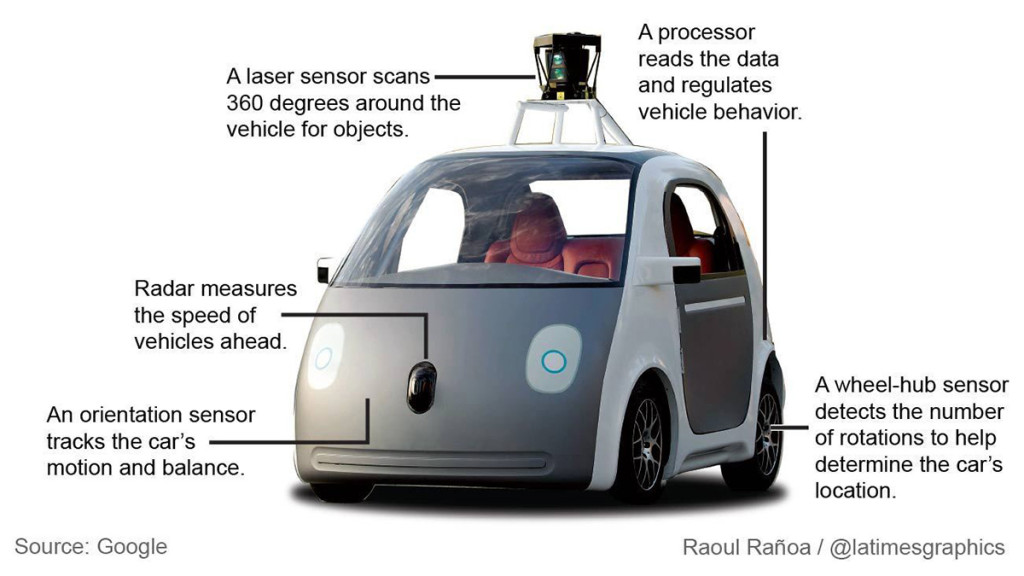
\includegraphics[width=10cm]{google_car.jpg}
					\caption{Google's Self-Driving Car}
				\end{center}
			\end{figure}

			Taking safety and other factors into account, the completely self-driving car is still in the testing phase and the government doesn't allow the vast majority of them to get onto ordinary roads. Considering its 	incomparable advantages compared to human-driving car, we will simulate and analyze its motion behavior as well as its interaction with other cars on highways.

		\subsection{Previous Research}
			Elliott Schwartz in Haverford College studied the effects on large-scale traffic flow of self-driving cars mixed in with human drivers. He found that when 80 percent of cars on the highway were self-driving, peak flow was approximately 24 percent higher than with only human drivers, and seriously congested flow did not occur until a density twice as high. Also he studied optimal behavior for self-driving cars and found that leaving a small gap when following cars close ahead, and checking behind when changing lanes to avoid cutting other cars off will contribute to the efficient transportation.

		\subsection{Restatement of the Problem}
			We are required to establish a model to analyze the effects on traffic flow of the number of lanes, peak and average traffic volume. Then we are expected to simulate the whole cooperating system under different percentage of vehicles using self-driving. In addition, we have to apply the model to the data for the specific roads, provided in the attached.

			In order to solve those problems, we will proceed as follows:

			\begin{itemize}
				\item \textbf{Stating assumptions.}

					By stating assumptions, we will simplify the problem and make it convenient for us to simulate real-life conditions.

				\item \textbf{Making notations, Definitions and Conventions}

					We give some notations which are necessary for us to clarify our models. After that, definitions and conventions about some terms are listed.

				\item \textbf{The model estabilish and test process}

					Actually, we use a model called Velocity - Dependent - Randomization (VDR) Model\scite{3} to simulate non-self-driving cars' behavior which is based on the Nagel - Schreckenberg Cellular Automata Model and improved by set the probability of drivers decelerate randomly is related with the traffic density and the ratio of $v_{i}$ and $v_{max}$.

					Then the difference between self-driving and non-self-driving car is that the self-driving car can maintain in the middle of the front car and the rear car automatically instead of being so close to the front one. Also, the self-driving car does't have the random deceleration phenomenon.

				\item \textbf{Sensitivity analysis.}


				\item \textbf{Result and further discussion.}

					After the conclusion, we consider whether some of lanes are dedicated to self-driving cars would make any change and test it with simulating  and comparing to the previous simulation. 

			\end{itemize}

	\section{Assumptions and Justifications}
		To simplify our models, we make the following basic assumptions, each of which is properly classified and justified.

		\textbf{Outside environment}
			\begin{itemize}
				\item The highway is flat and divided in to different parts. The highway is obstacle-free with constant speed: limit $v_{max}$.

				\item The assumption of highway is if there are no particular cases, all the vehicles driving at their maximum speed (no more than $v_{max}$).

				\item The assumption of traffic rules exist which constrain the vehicles extremely. In another word, each vehicles, regarding to self-driving or non-self-driving, follows the rules so that in highway, notionally at least, the probability of accident is zero.

				\item The assumption of highway is each cars should drive in the fixed direction in a particular highway. U-turn and taking a sudden turn are not allowed.

				\item The highway is also divided into interstate and state highway. The assumption is that the difference between them is the limit speed besides the length, width and so on.
			\end{itemize}

		\textbf{Vehicles condition}
			\begin{itemize}
				\item As the assumption before ,each car drives at its maximum speed. But when it should be considered that the percentage of errors is added, we assume that the probability of accident is still zero (It will cause severe traffic jam or larger accidents, which we can not control), but the probability of traffic jam is becoming higher.

				\item A car’s position is determined by a lane number and a horizontal position. Thus, on a stretch of road with n operating lanes, the position of a car is given by the ordered pair $(x, i)\in R \times \{1, 2, . . . , n\}$. (Cellular Automate Simulation)

				\item Vehicles are of constant length.
			\end{itemize}

		\textbf{Driving behavior}
			\begin{itemize}
				\item Cooperating system is between the self-driving and self-driving or self driving and non-self driving. Drivers do not cooperate. While the drivers are not directly competing against one other, they are affecting each other and are hence fierce indirect obstacles/opponents.

				\item Self-driving system in cooperating cars is an excellent automatic system with the fixed error percentage.

				\item When the front car stops, the car behind have two choice: stop and wait or change an other lane. But we should notice if cars all stop, it will be a traffic jam. We encourage most vehicles to change ways however with the error possibility exists, vehicles changing lanes also causes the traffic jam. So we assume this probability is lower than it when stop.

				\item We use volume to analyze the efficiency of cooperating system. The assumption is the traffic flow in all ordinary hours is steady and smooth and so is the peaking hours.
			\end{itemize}

	\section{Notations}
		The following table provides meanings of important notations used in our models and simulations.
		\begin{table}[H]
			\caption{Notations}
			\begin{center}
				\begin{longtable}{m{80pt}<{\centering} m{260pt} m{50pt}}
					\hline
					%---------------------------------------------------------------------------------
					Symbols 		& 	Definition 										& 	Unit		\\
					\hline
					%---------------------------------------------------------------------------------
					ID 				& 	Route ID 										& 	unitless	\\
					SM 				& 	Start Milepost 									& 	unitless	\\
					EM 				& 	End Milepost 									& 	unitless	\\
					L 				& 	Lane length										& 	mile 	 	\\
					$N_{L}$ 		& 	Number of Lanes 		 						& 	lanes 		\\
					$n_{1}$ 		& 	Number of self-driving lane DECR MP direction 	& 	lanes 		\\
					$n_{2}$ 		& 	Number of self-driving lane INCR MP direction 	& 	lanes 		\\
					W 				& 	Lane width 										& 	ft 			\\
					$S_{n}$ 		& 	Size of non-self-driving car 					& 	m 			\\
					$S_{s}$ 		& 	Size of self-driving car 						& 	m 			\\
					$V_{max}$ 		& 	Limit speed 									& 	mile/h 		\\
					$\rho$ 			& 	Traffic density 								& 	cars/h 		\\
					$T_{0}$ 		& 	Peaking hour 									& 	h 			\\
					$P_{i}$ 		& 	Percentage of self-driving 						& 	unitless 	\\
					$H_{i}$ 		& 	Distance between cars 							& 	m 			\\
					C 				& 	Daily traffic counts 							& 	cars 		\\
					$d_{2}(dummy)$ 	& 	Self-driving/non-self-driving 					& 	unitless 	\\
					\hline
					%---------------------------------------------------------------------------------
				\end{longtable}
			\end{center}
		\end{table}
		Although we directly using the unit given by problem instead of unify the units in the table above, we will convert the units into SI units in the later calculations and simulations.

		There are some of the notations are defined later.

	\section{Definitions and Conventions}

		\begin{itemize}
			\item \textbf{Cars} are divided in two main types: one is self-driving cars and the other is non-self-driving cars, which contain different sizes .

			We conclude cars in three sizes: small (cars), medium (coaches), large (trucks), which have different distances between each other. The rule is the larger the size is, the longer the distance there will be.

			\item \textbf{Self-driving\&non-self-driving} are two styles of driving in this essay. Non-self-driving cars are the traditional styles of cars in our daily life, which are wholly operated by human beings.

			With the rapid development of technology, self-driving cars is becoming more and more popular.

			Self-driving cars are smart, automatic mechanism. They can drive by themselves without any operation according to their “Cooperating System” which could detect the surrounding objects as well as react to behave directly.

			\item \textbf{Peaking hour} is a period of time when more vehicles choose to pass the highway. We use the data “8\% of the daily traffic volume occurs during peak travel hours” and calculate below:

			\begin{equation}
				T_{0} \leq 8\%\times24h = 1.92h
			\end{equation}

			When the peaking hour equals to 1.92 hours ,the volume of peaking hour is same with the volume of average hour. So we fix the peaking hour as 1.5 hours.
		\end{itemize}

	\section{The Standard Nagel - Schreckenberg Cellular Automata Model}
		\noindent \textbf{The timing diagram}

			Based on the standard N-S model, we can easily find the relationship between time and the position of each car which can be shown by a timing diagram.
			\begin{figure}[H]
				\begin{center}
					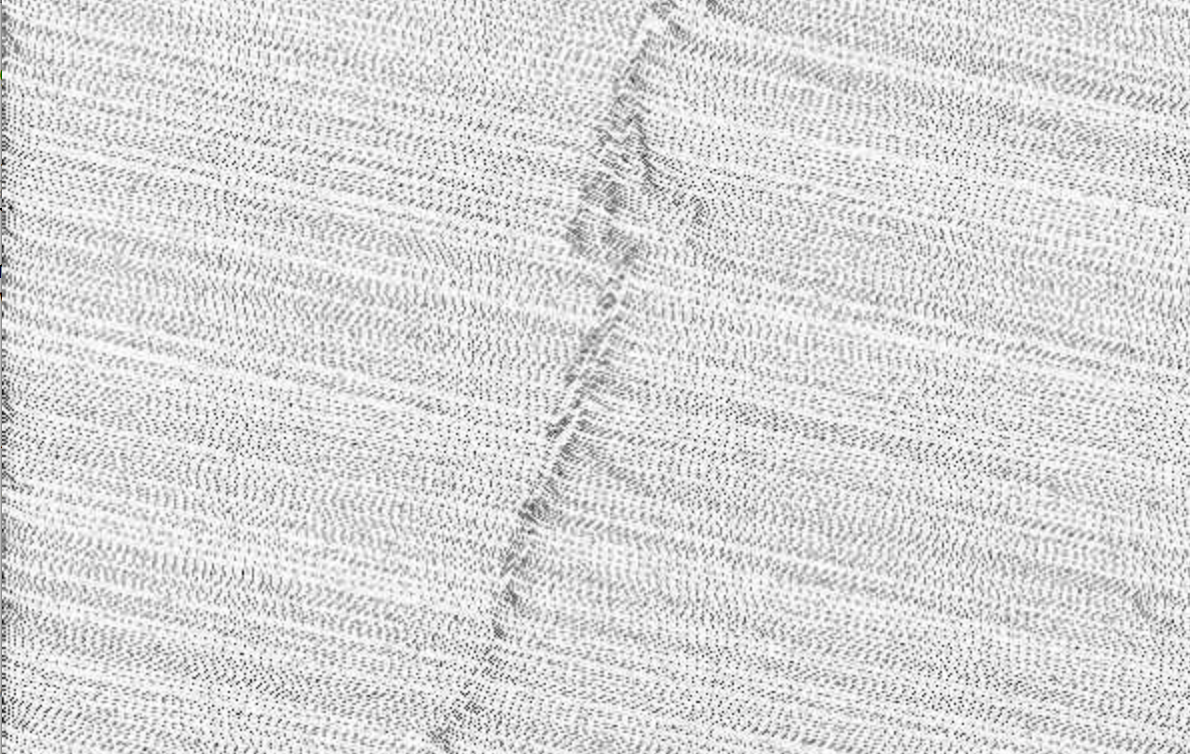
\includegraphics[width=12cm]{timing.png}
					\caption{The timing diagram}
				\end{center}
			\end{figure}

			The car entries from left and travel out from the right, the time change from upside to downside. With the timing diagram, we can figure out the road condition intuitively and much easier to deal will multi-lanes situation.
		\subsection{Multi-lanes non-self-driving}
			A lane is a large set of cells which combine together with equal length. Each cell is approximately 7.5 meters long and contains information about whether it contains a car. Multi-lanes represent arrays of lanes described $L \times N_{L}$. When initialized, this array contains empty grid spaces\scite{4}. If it is occupied, we get certain information that cars enter in grid spaces are activated and infused with information about the cars. Then, with this information, the state of the system at the next time step can be determined. Moreover, we use speed number to replace the number of whether the cell is occupied by a car.
			\begin{equation}
				Array=
				\begin{bmatrix}
					0&1&0&3&0&0&2&0&4\\
					2&0&3&0&1&4&0&1&0
				\end{bmatrix}
			\end{equation}
			\begin{itemize}
				\item The speed of the car was a random number selected in $\{0, 1, 2, 3, \cdots, v_{max}\}$.\\

				The average speed is:$\bar{v} = \frac{\Sigma v_{i}}{N_{car}}$
				\item From proceed of $t \rightarrow t+1$, the fundamental N-S model gives several rules to generate.
			\end{itemize}

			\textbf{Step 1: Acceleration}

				If the speed of car $v_{i}$ is lower than $v_{max}$, the car has the tendency to speed up to the $v_{max}$. 

			\textbf{Step 2: Deceleration}

				The speed of car will slow down when the front gap is not satisfied the current speed. The speed will decrease to $gap_{i}$.

			\textbf{Step 3: Randomization}

				In non-self-driving car model, the drivers decrease the speed randomly. If the $v_{i}>0$, the speed of $car_{i}$ will reduce with the probability $\lambda_{random}$.

				We fix the deceleration parameter $\lambda_{random}=0.25$

			\textbf{Step 4: Move}

				The new position of the car is determined by the current velocity and position.

				Assume that the percentage of entry $\lambda_{in}=0.2$

			\textbf{Step 5: Changing lane}

				In two-lane traffic, cars will switch lanes when the following conditions are satisfied:
				\begin{itemize}
					\item The distance ahead in current lane is smaller than the car speed.
					\item The distance ahead in another lane is larger than in the current lane.
					\item There exists an empty cell right in another lane.
					\item The distance ahead of the following vehicle in another lane is larger than the speed of the following vehicle
						N-S model simplified probability of changing lane into a fixed parameter $\lambda_{H\_switch} = 0.25$
				\end{itemize} 

				We assume that all the single-lane rules are still suitable in multi-lanes model. 		

		\subsection{Multi-lanes self-driving}
			We have assumed that the self-driving car is intelligent enough to choose its speed. And it will follow the ordinary rule of N-S model except:
			\begin{itemize}
				\item The probability of switching lane will larger than it of non-self-driving car. Under the premise of security, the self-driving car will choice the most effective way to pass without "hesitate" like human drivers. Taking into account other random factors, we set the probability of self-driving switching lane is:
				\begin{equation}
					\lambda_{A\_switch} = 0.75
				\end{equation}
				\begin{figure}[H]
					\begin{minipage}[H]{0.5\linewidth}
						\centering
						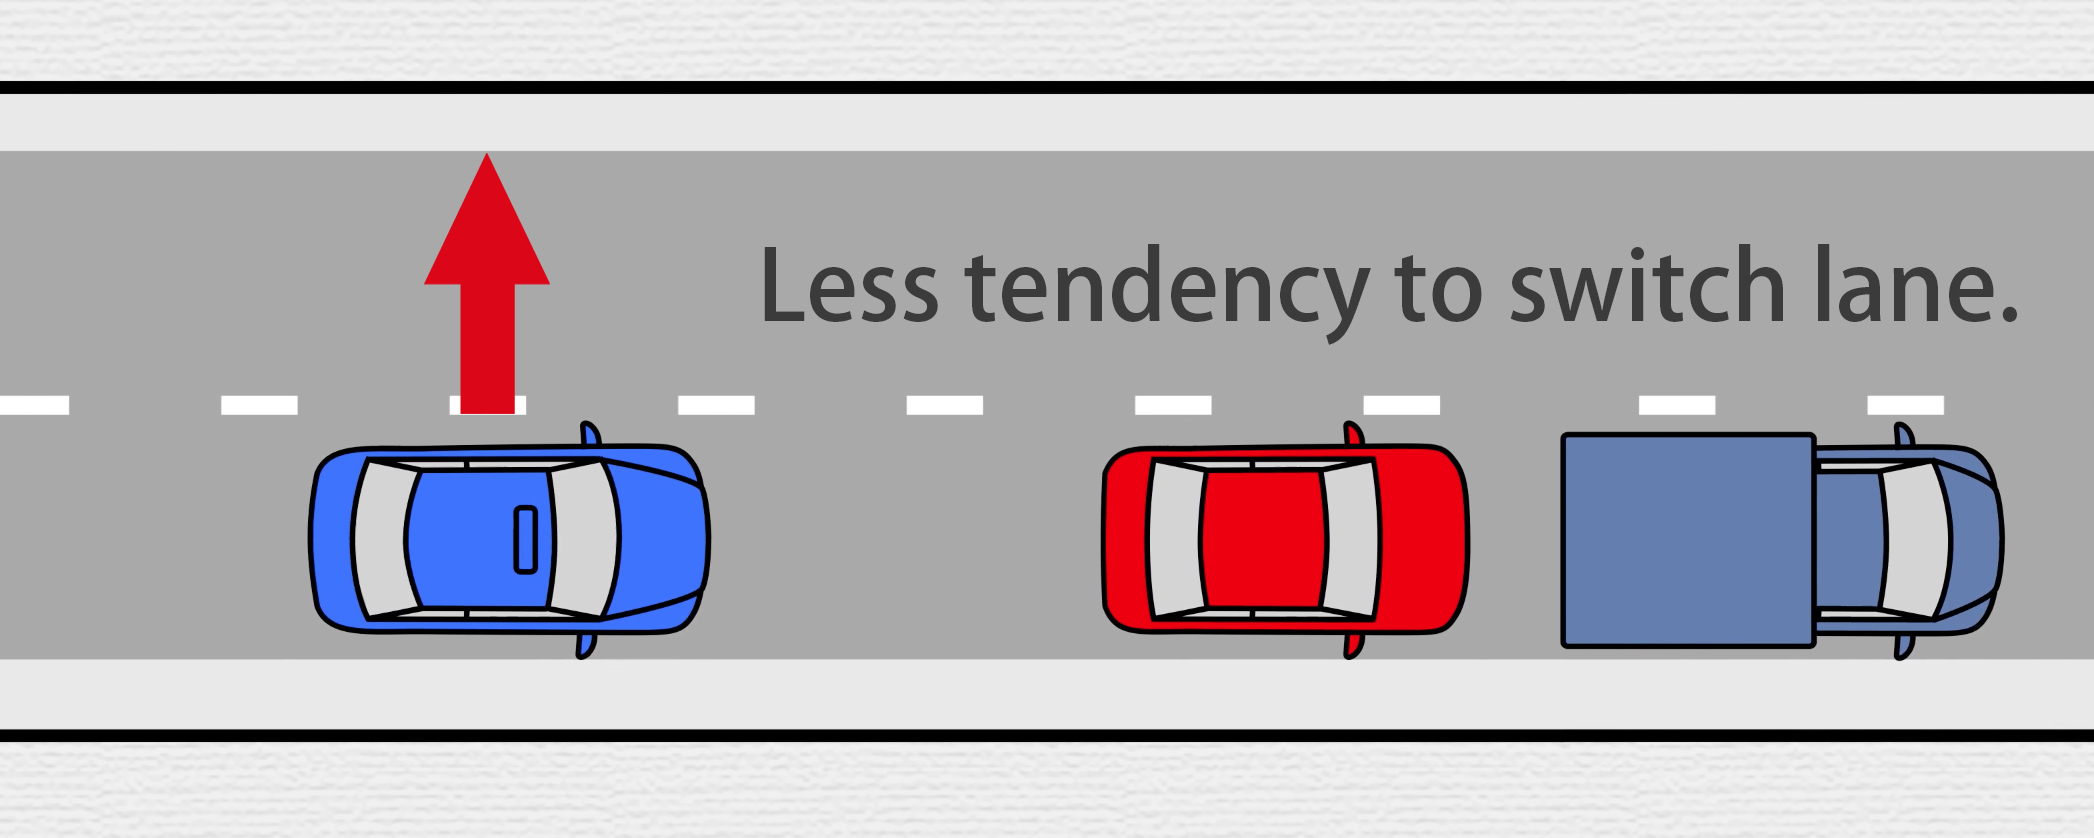
\includegraphics[width=7cm]{non-switch.jpg}
						\caption{Non-self-driving car switching}
					\end{minipage}%
					\begin{minipage}[H]{0.5\linewidth}
						\centering
						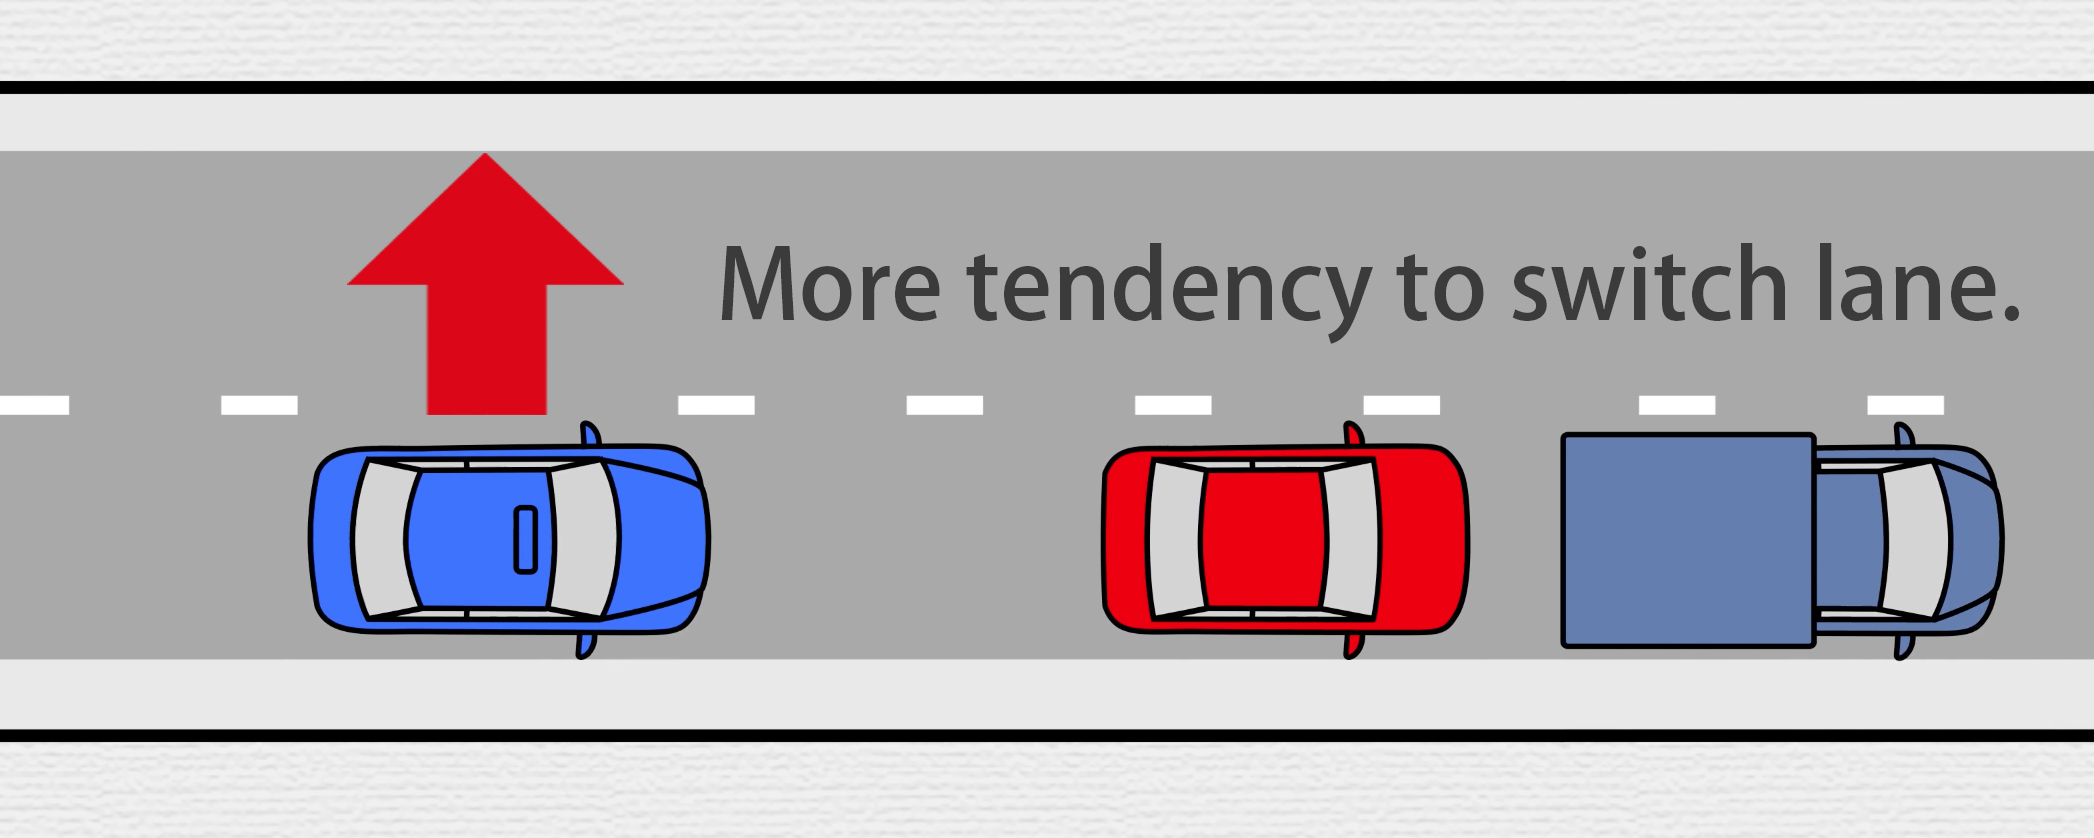
\includegraphics[width=7cm]{self-switch.jpg}
						\caption{Self-driving car switching}
					\end{minipage}
				\end{figure}
				\item A self-driving car is able to detect surrounding cars and maintain in the middle of the front car and the rear car automatically instead of being so close to the front one.
				\begin{figure}[H]
					\begin{minipage}[H]{0.5\linewidth}
						\centering
						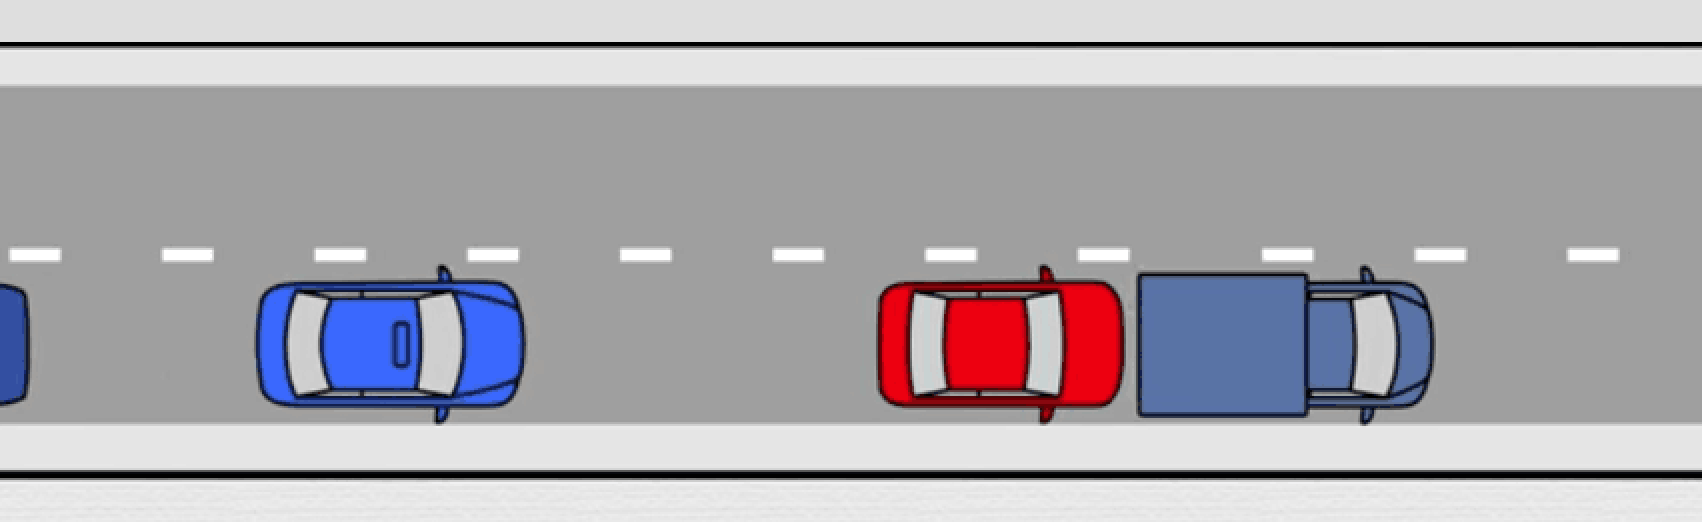
\includegraphics[width=7cm]{non-self.png}
						\caption{Non-self-driving car\protect\\front and back distance}
					\end{minipage}%
					\begin{minipage}[H]{0.5\linewidth}
						\centering
						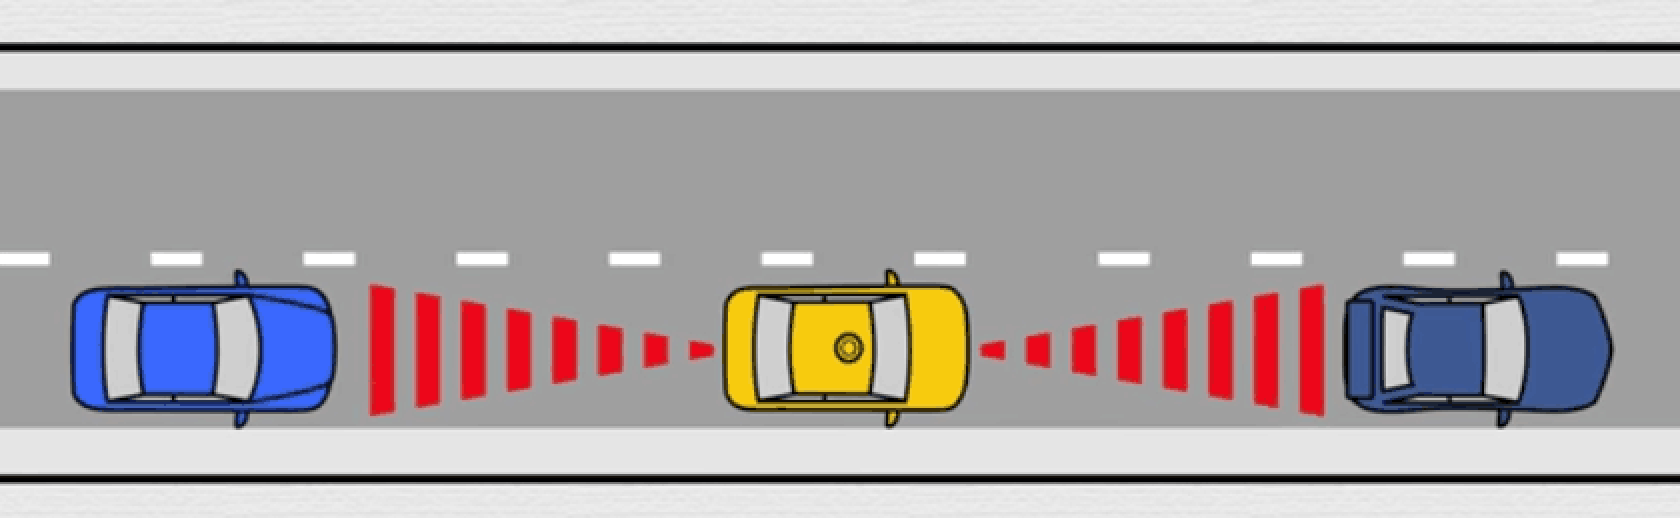
\includegraphics[width=7cm]{self.png}
						\caption{Self-driving car\protect\\front and back distance}
					\end{minipage}
				\end{figure}
				\item The self-driving car doesn't have the possibility to decelerate randomly.
				\begin{equation}
					\lambda_{random}=0
				\end{equation}
			\end{itemize}


	\section{The Real Road Traffic Condition}
		We select Route5 as an example to analyze the real situation of traffic flow. Assume that the other four highways suit the same situation of Route5.

		Calculate the data from sheet and get the figure below:
		\begin{figure}[H]
			\begin{center}
				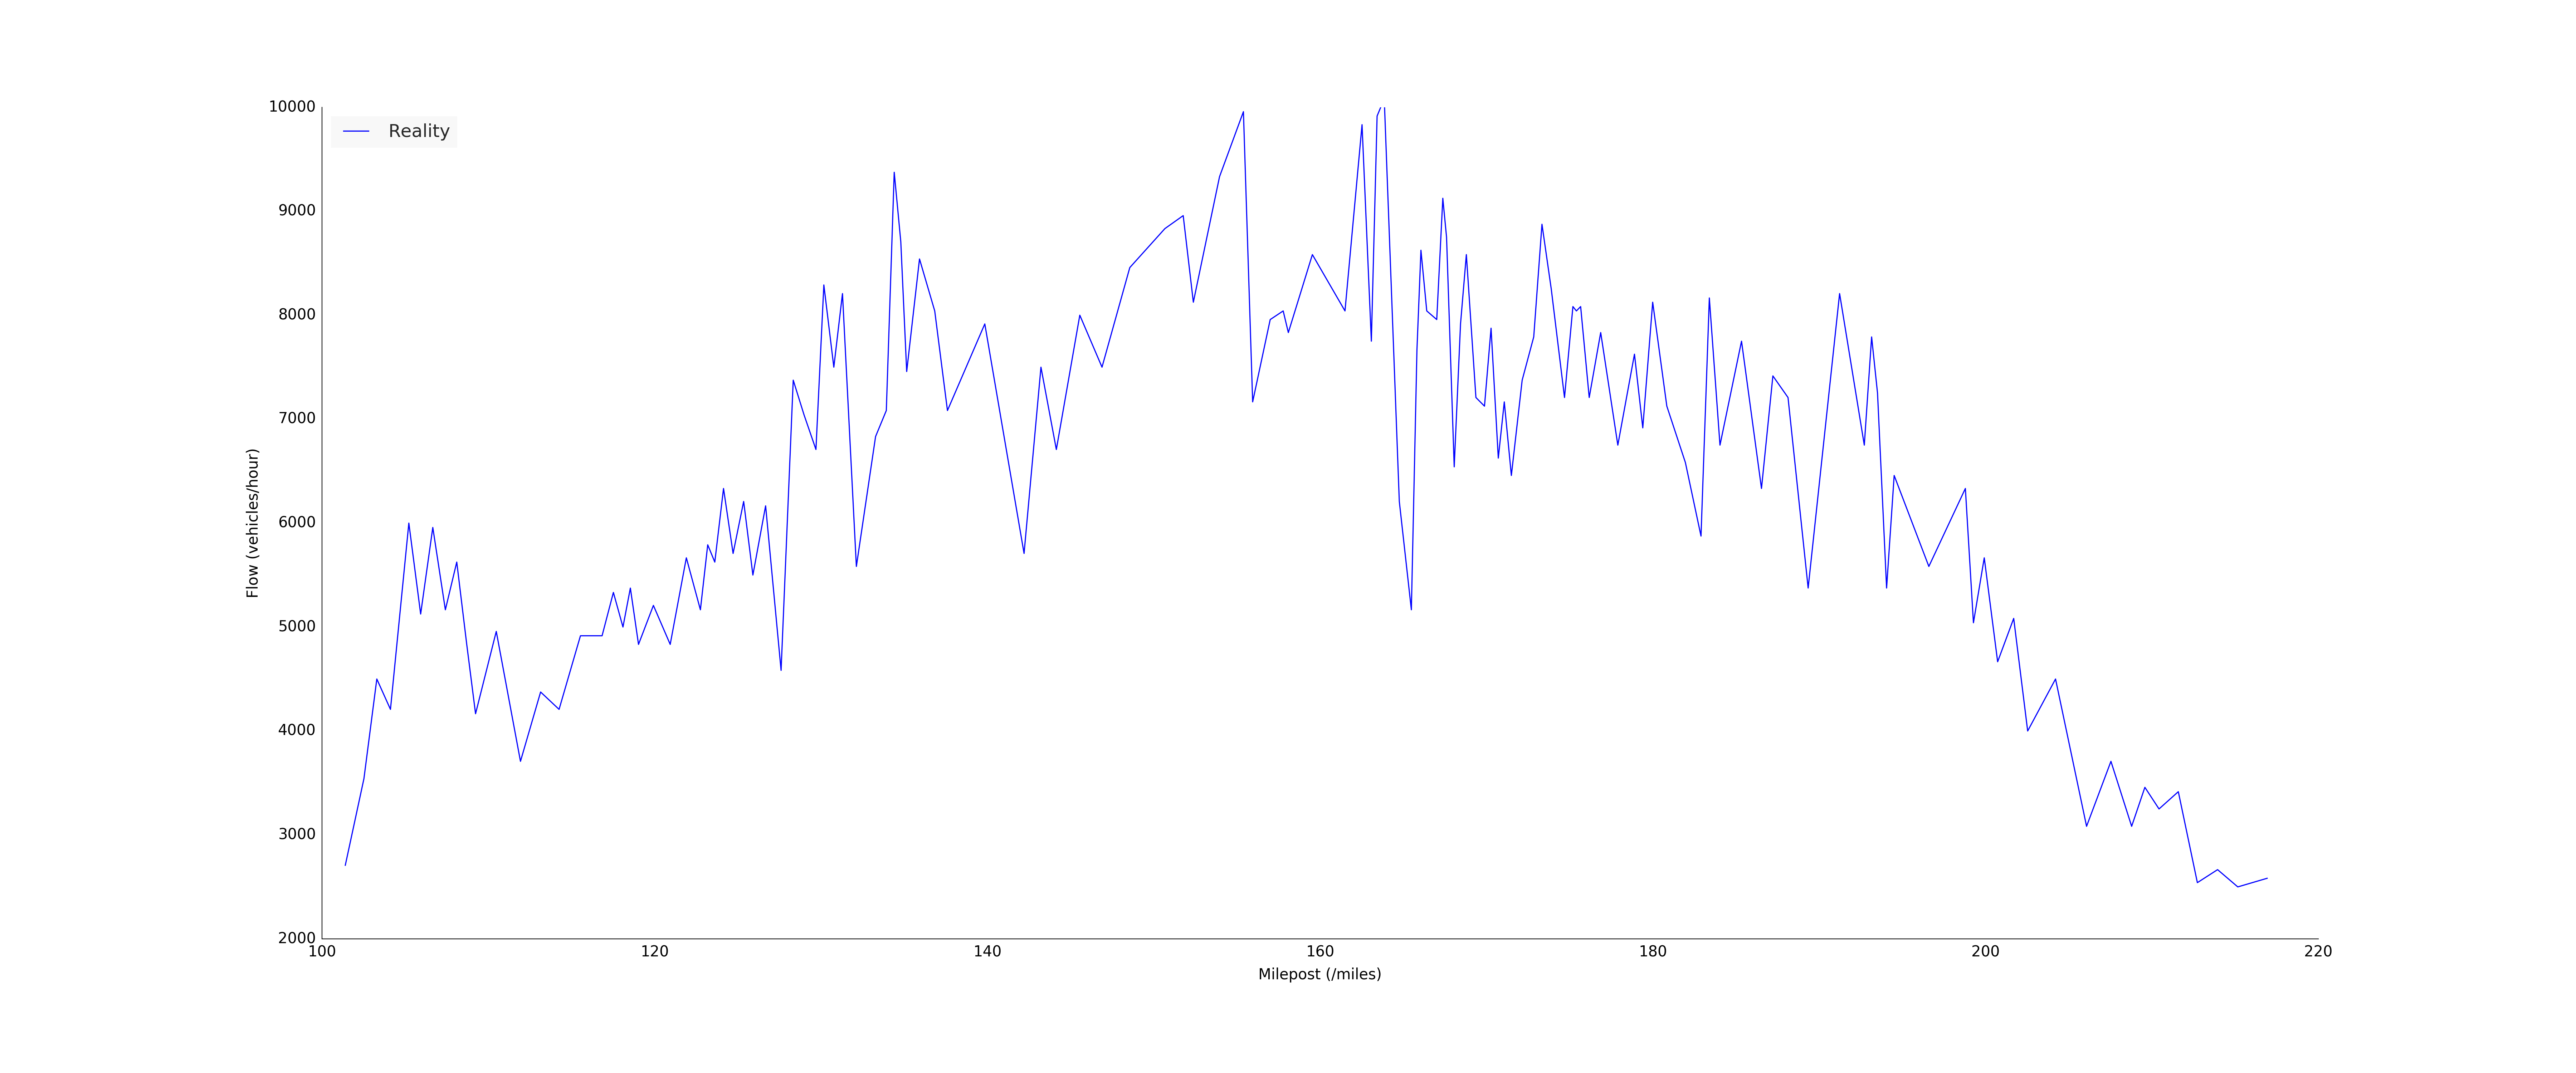
\includegraphics[width=15cm]{r5.png}
				\caption{The real traffic condition of Route5}
			\end{center}
		\end{figure}

		Fit our model to satisfy the curve showing below:
		\begin{figure}[H]
			\begin{center}
				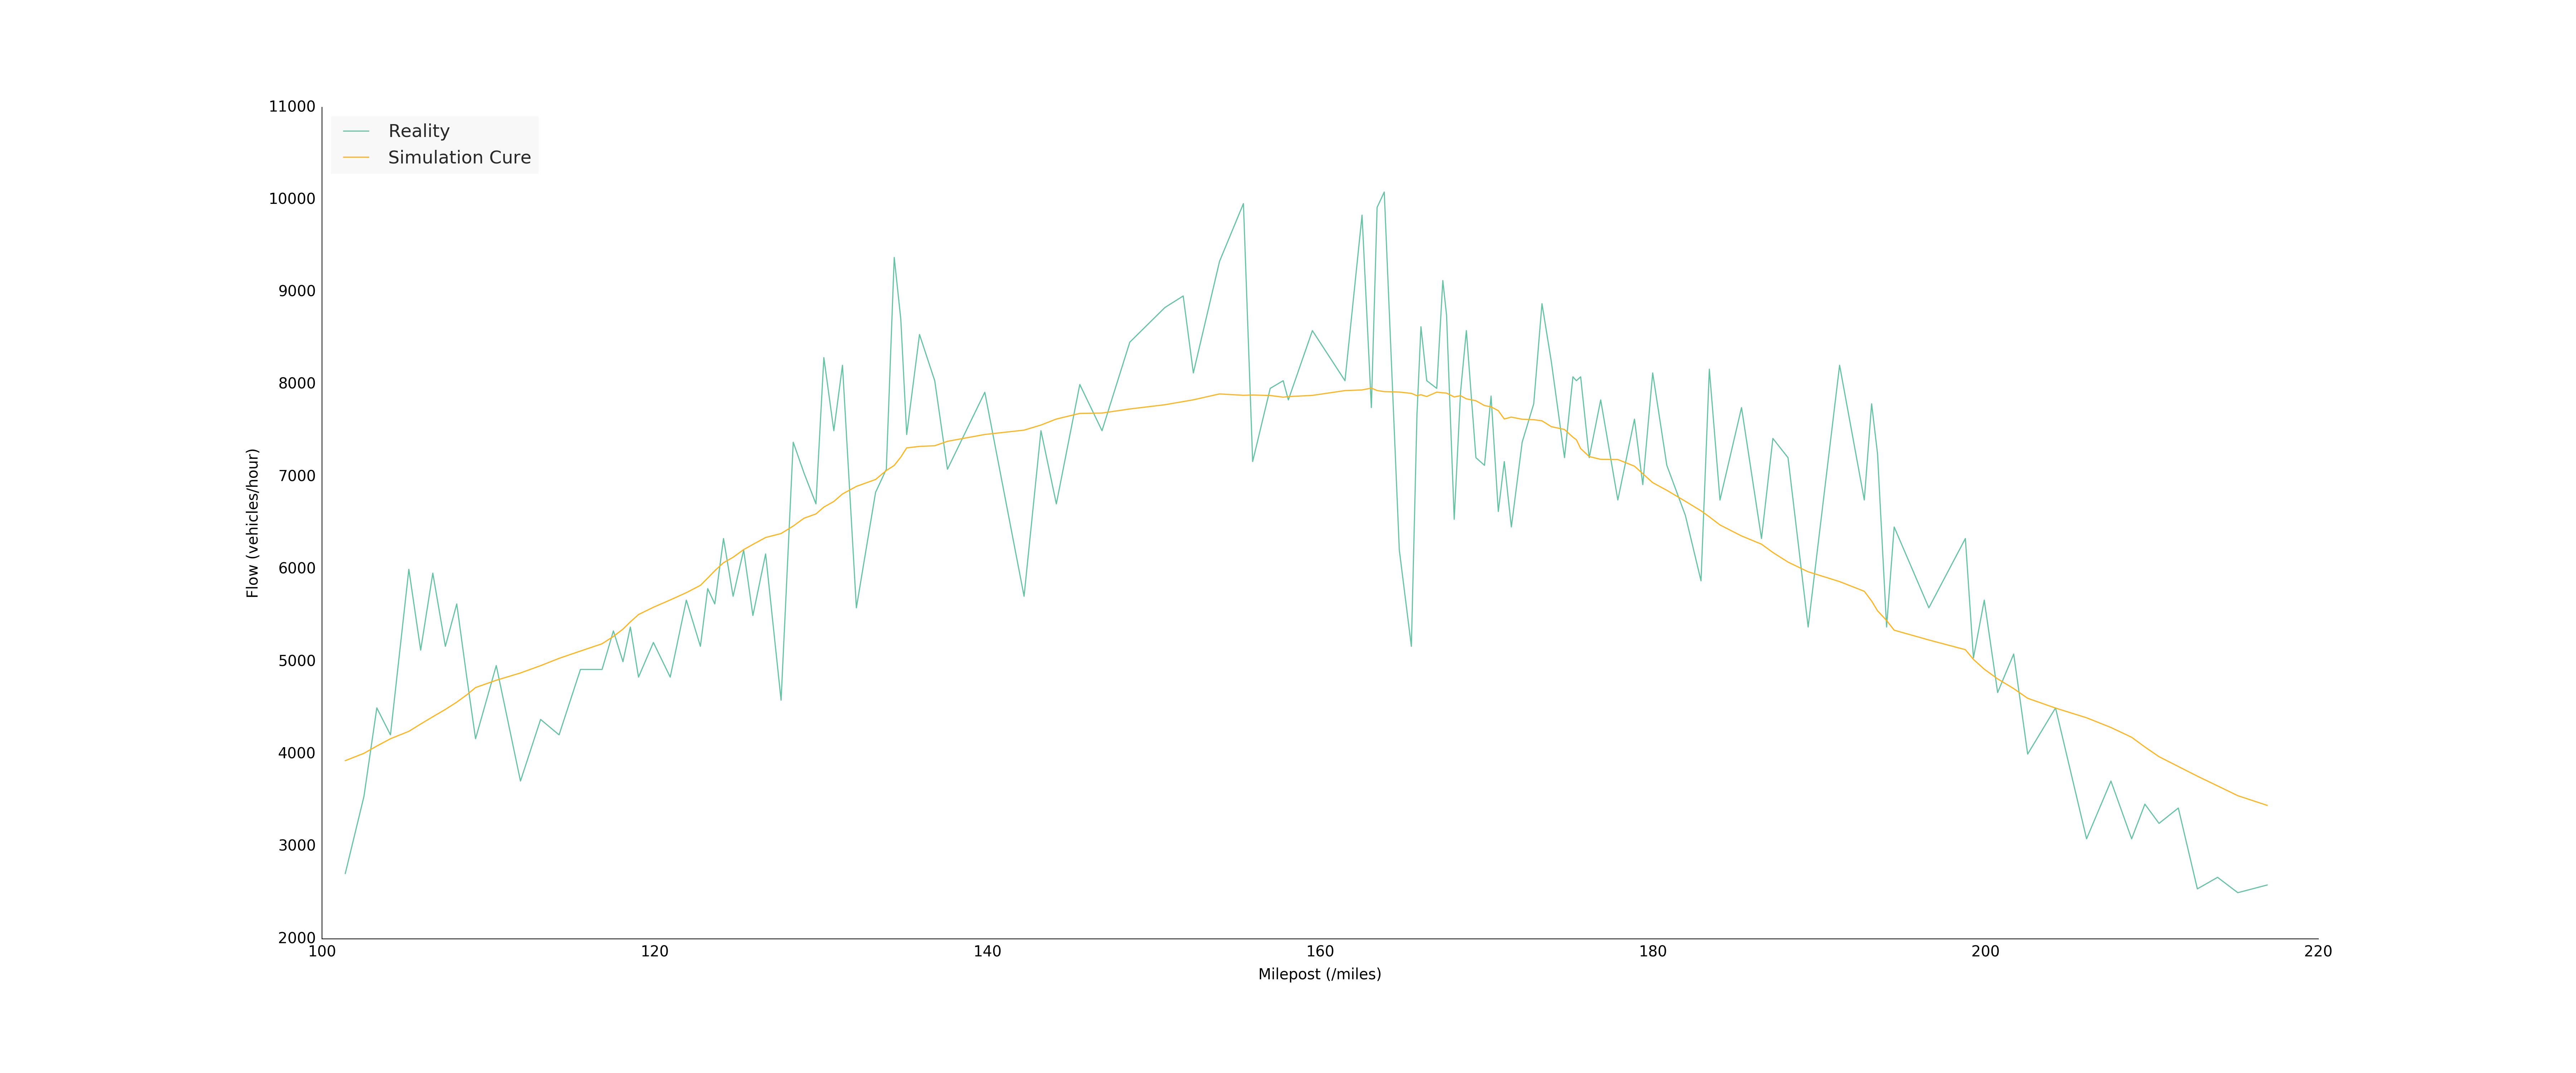
\includegraphics[width=15cm]{r51.png}
				\caption{The simulation of traffic condition of Route5}
			\end{center}
		\end{figure}

		We find that it is difficult to fix the real condition. It is obvious that we do not consider some important factors in our model.


	\section{Modified Model}
		\subsection{Modified VDR Model}
			In order to be more similar to the real traffic, based on the VDR model, a improved version of standard N-S model, we further optimize our model according to reality and common sense.
			\subsubsection{Non-self-driving car}
				\noindent \textbf{Randomization}

					According to standard N-S Model, a driver will slowdown randomly at a fixed probability. However, based on practical experience, the probability will be influenced by traffic condition. In order to embody this phenomenon, we define the probability is related to traffic density and the ratio of $v_{i}$ and $v_{max}$, regardless of the emotion of drivers and the fundamental situation of the highway(friction, weather, barrier etc.). The rule is given as:
					\begin{equation}
						v_{i} \rightarrow max (v_{i}-1, 0) 
					\end{equation}
					\begin{equation}
						\text{with} \quad \lambda_{random} = \begin{cases} p_{0}, &v_{i}=0\\ \ \\ \rho^{\beta \frac{v_{i}}{v_{max}}}&v_{i}>0\end{cases}
					\end{equation}
						
				\noindent \textbf{The inflow percentage}

					The standard N-S Model regards the inflow percentage $\lambda_{in}$ in the section of simulating road as a fixed value. We correlate the inflow percentage with 3 different factors including: whether it is during peaking hour, whether it is on a interstate route or state route and whether there is a junction nearby. 
					\begin{equation}
						\lambda_{in} =  \epsilon_{peaking}D_{peaking} + \epsilon_{interstate}D_{interstate} + \epsilon_{junction}D_{junction}
					\end{equation}
					\noindent When it is during peaking hour, the binary variable $D_{peaking}$ is 1 or $D_{peaking}$ is 0.\\
					When it is on a interstate route, the binary variable $D_{interstate}$ is 1 or $D_{interstate}$ is 0.\\
					When it is a junction nearby, the binary variable $D_{junction}$ is 1 or $D_{junction}$ is 0.

					Then, we discuss these 3 influencing factors respectively. 
					\begin{itemize}
						\item \textbf{Peaking hour or not}\\
							When fix the other 2 factors and focus on whether it is during peaking hour, we draw a conclusion that the traffic flow is large than that in ordinary hour with the increase of milage. 
							\begin{figure}[H]
								\begin{center}
									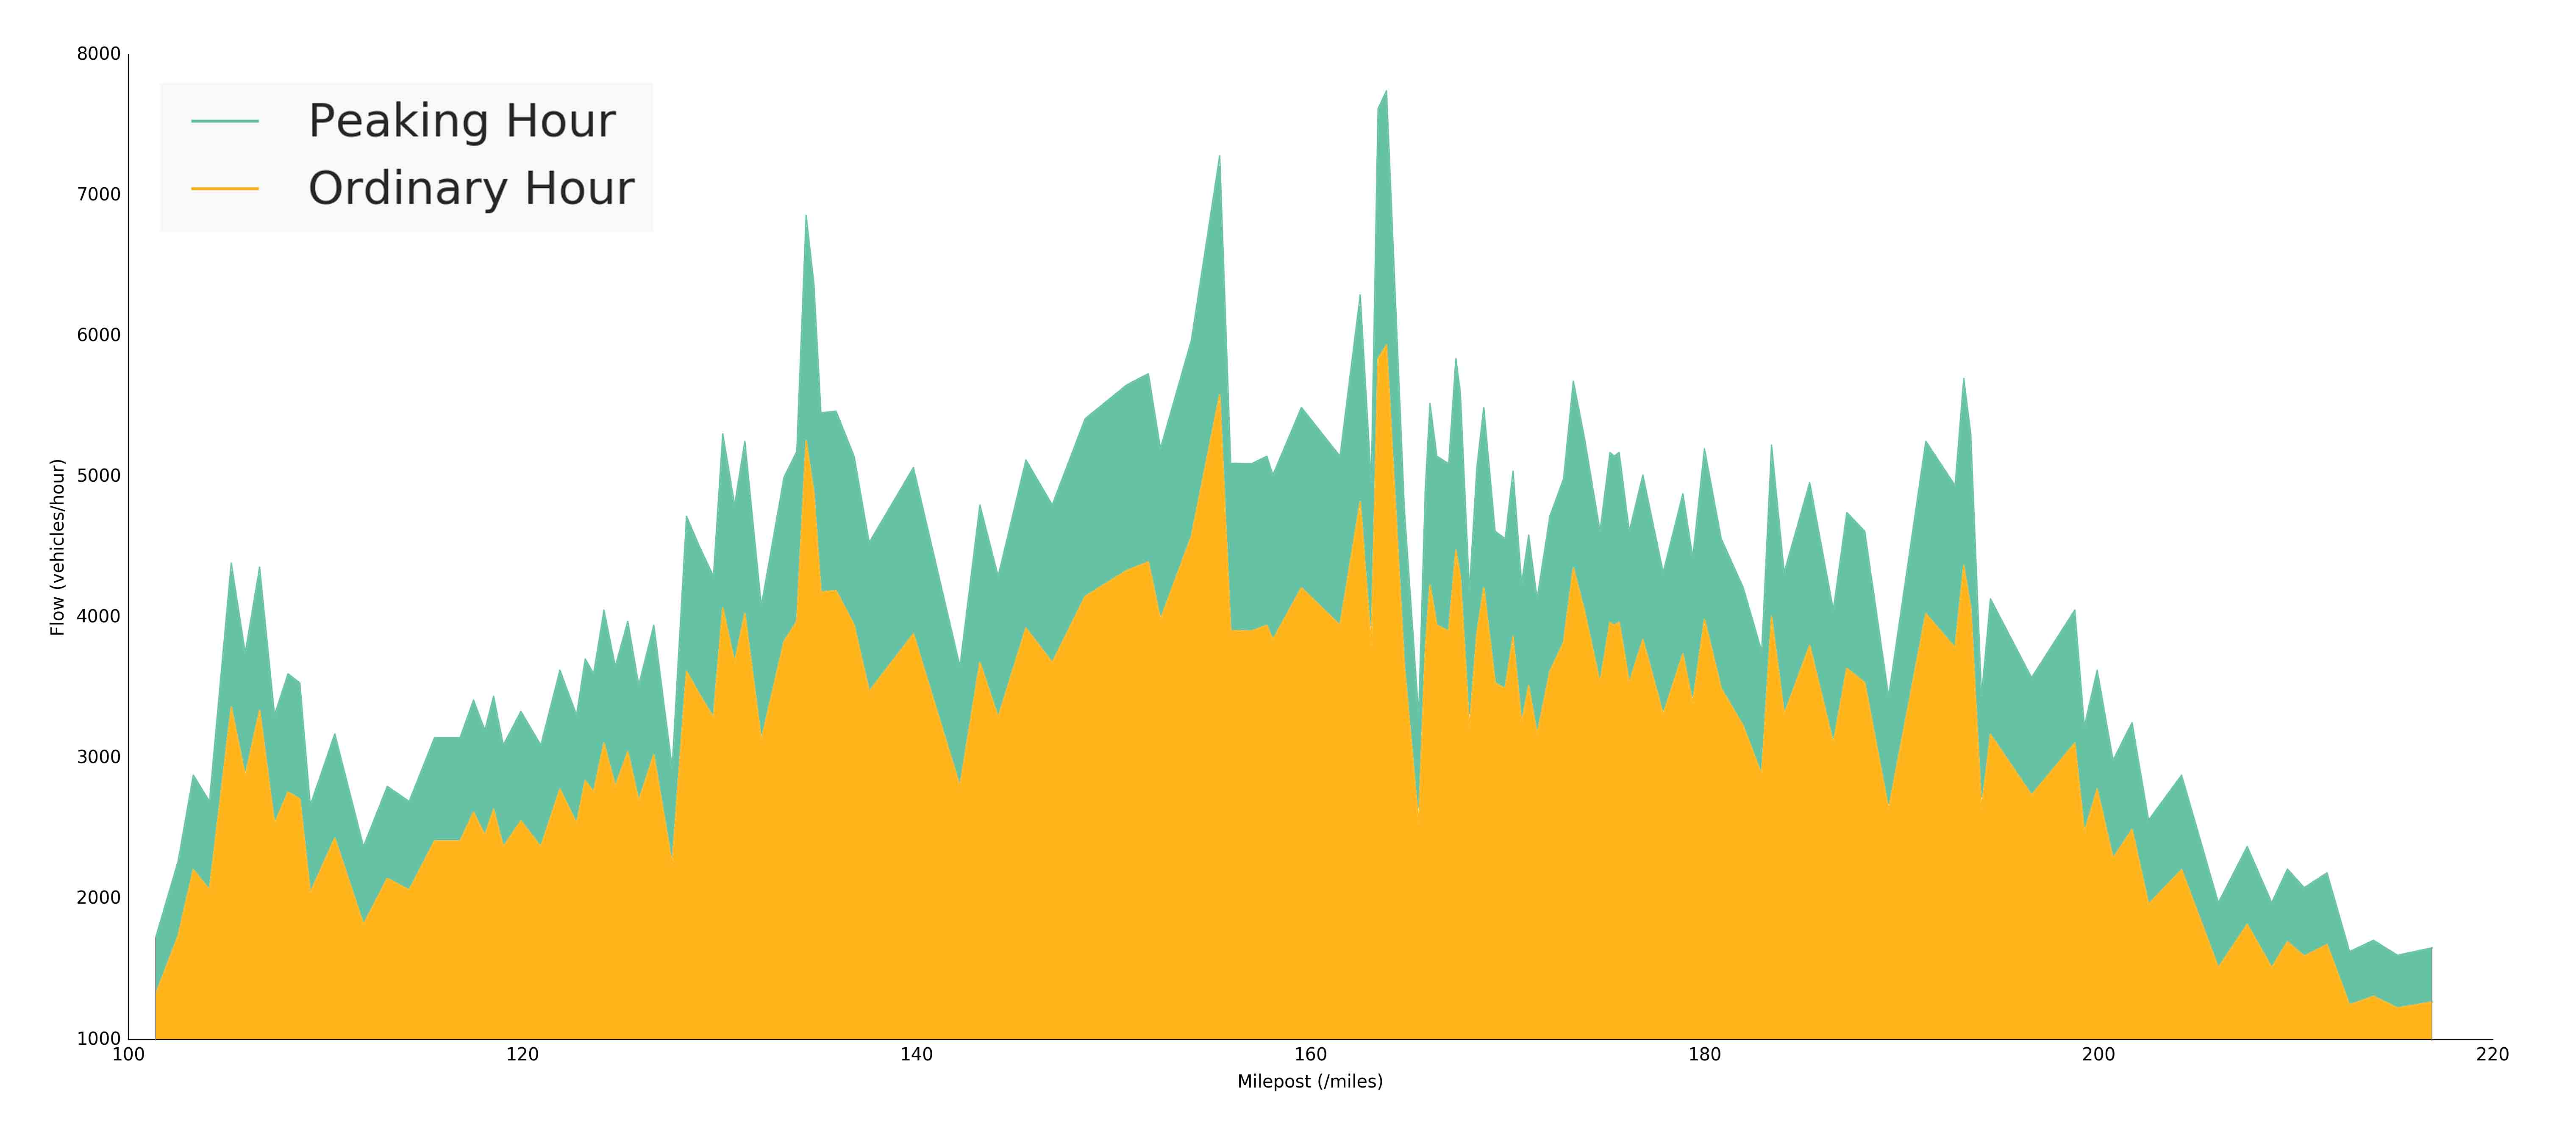
\includegraphics[width=12cm]{milepost.jpg}
									\caption{Peaking hour effect}
								\end{center}
							\end{figure}
						\item \textbf{Interstate route or not}\\
							Then comes to whether it is on a interstate route. It is well known that the traffic flow on interstate routes is larger than that on state routes. So this factor would obviously affect the inflow percentage of the section of road we simulating on.
						\item \textbf{A junction nearby}\\
							Finally, if there is a junction nearby, it will have a obvious effect on the traffic flow on the road as the folk on the road can bring in or move away some of the cars. \\
							We set a growth/attenuation coefficient $\gamma_{i}$ to measure the influence of a junction on the traffic flow.
							\begin{equation}
								\gamma_{i}=\frac{Flow_{junc}}{Flow_{near}}
							\end{equation}
							The $Flow_{junc}$ is the traffic flow on the section of road where there is a junction. $Flow_{near}$ is the traffic flow on the road near the previous section.

							Through the data processing, we list a table of different value of $\gamma_{i}$ with the increase of milage. 
							\begin{table}[H]
								\caption{The value of $\gamma_{i}$}
								\begin{center}
									\begin{longtable}{| m{60pt}<{\centering} | m{60pt}<{\centering} | m{60pt}<{\centering} | m{60pt}<{\centering} | }
										\hline%------------------------------------------------------------
										$\gamma_{i}$	& 	value	& 	$\gamma_{i}$ 	& 	value	\\
										\hline%------------------------------------------------------------
											1			&	1.43	&		6 			&	1.15	\\
										\hline%------------------------------------------------------------
											2			&	0.75	&		7			&	1.15	\\
										\hline%------------------------------------------------------------
											3			&	0.74	&		8			&	0.62	\\
										\hline%------------------------------------------------------------
											4			&	0.68	&		9			&	0.75	\\
										\hline%------------------------------------------------------------
											5			&	1.04	&		10			&	0.92	\\
										\hline%------------------------------------------------------------
									\end{longtable}
								\end{center}
							\end{table}

					\end{itemize}
				\noindent \textbf{Result}

					Taking these factors into consideration, we get the ameliorative result as the figure below.
					\begin{figure}[H]
						\begin{center}
							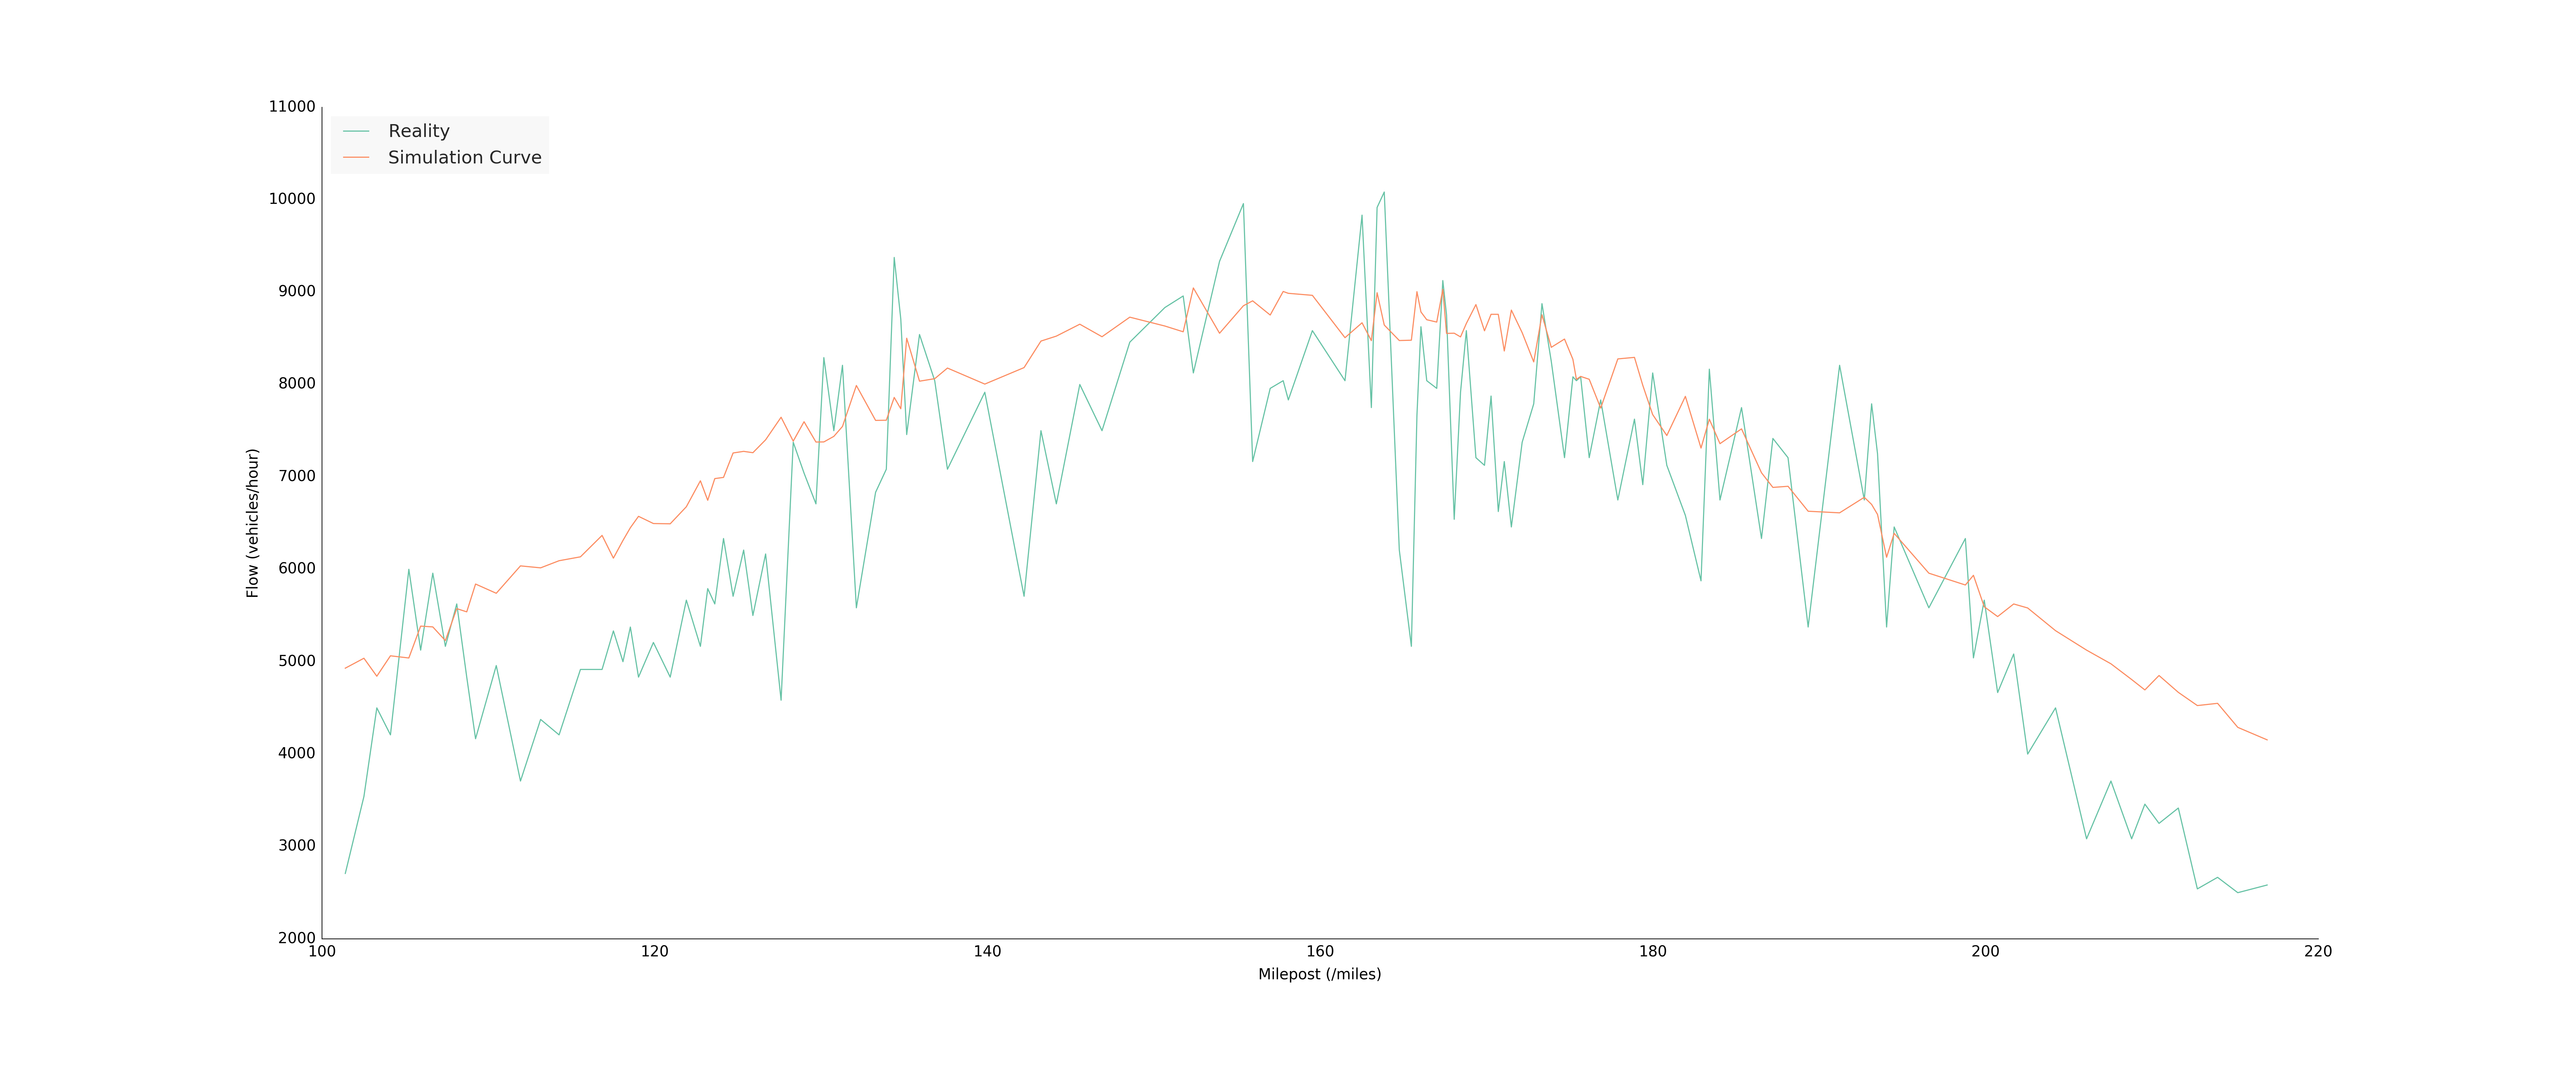
\includegraphics[width=15cm]{r52.png}
							\caption{The simulation of traffic condition of Route5 after modifying}
						\end{center}
					\end{figure}
			\subsubsection{Self-driving car}
				\noindent \textbf{The cooperating system}

					We assumed that the self-driving car is intelligent enough and has a cooperating system which will interact with non-self-driving car and cooperate with self-driving car.
					\begin{itemize}
						\item If a self-driving car detects the leading car is non-self driving, it will maintain a relatively Long distance to the leading one, just a little shorter than the normal vehicle distance. 
						\item On the contrary, if it detects there is also a self-driving car in front of itself,  the rear one may adjust its speed and the distance to the front car and finally get really close to it and have the same speed. Like the 2 self-driving cars are linked with each other. 
					\end{itemize}
					According to the description above, the self-driving car is able to conclude a Information set based on the surrounding circumstance which can be defined as follows:
					\begin{equation}
						I = \{ D_{F}L_{F} ,\ D_{L} ,\ D_{LF}L_{LF} ,\ D_{LB}L_{LB} \}
					\end{equation}
					\begin{table}[H]
						\caption{Definitions to the parameters in the Information set}
						\begin{center}
							\begin{longtable}{m{80pt}<{\centering} | m{240pt}}
								\hline%---------------------------------------------------------------------
								Parameter 	& 	Definition 												\\
								\hline%---------------------------------------------------------------------
								$D_{F}$ 	&	Whether the front car is self-driving.					\\
								\hline%---------------------------------------------------------------------
								$L_{F}$		&	The behavior of the front car.							\\
								\hline%---------------------------------------------------------------------
								$D_{L}$		&	Whether there is a car to the left/right of itself.		\\
								\hline%---------------------------------------------------------------------
								$D_{LF}$	&	Whether the left/right-front car is self-driving.		\\
								\hline%---------------------------------------------------------------------
								$L_{LF}$	&	The behavior of the left/right-front car.				\\
								\hline%---------------------------------------------------------------------
								$D_{LB}$	&	Whether the left/right-back car is self-driving.		\\
								\hline%---------------------------------------------------------------------
								$L_{LB}$	&	The behavior of the left/right-back car.				\\
								\hline%---------------------------------------------------------------------
							\end{longtable}
						\end{center}
					\end{table}
				\noindent \textbf{The changes caused by the percentage of self-driving car}

					Because of the cooperation and interation system of the self-driving car, the road capacity will certainly enlarged with the increasing of the percentage of self-driving car.


			\subsubsection{Comparison of non-self-driving and self-driving}
				\noindent \textbf{Comparison in time-velocity}
					\begin{figure}[H]
						\begin{minipage}[H]{0.5\linewidth}
							\centering
							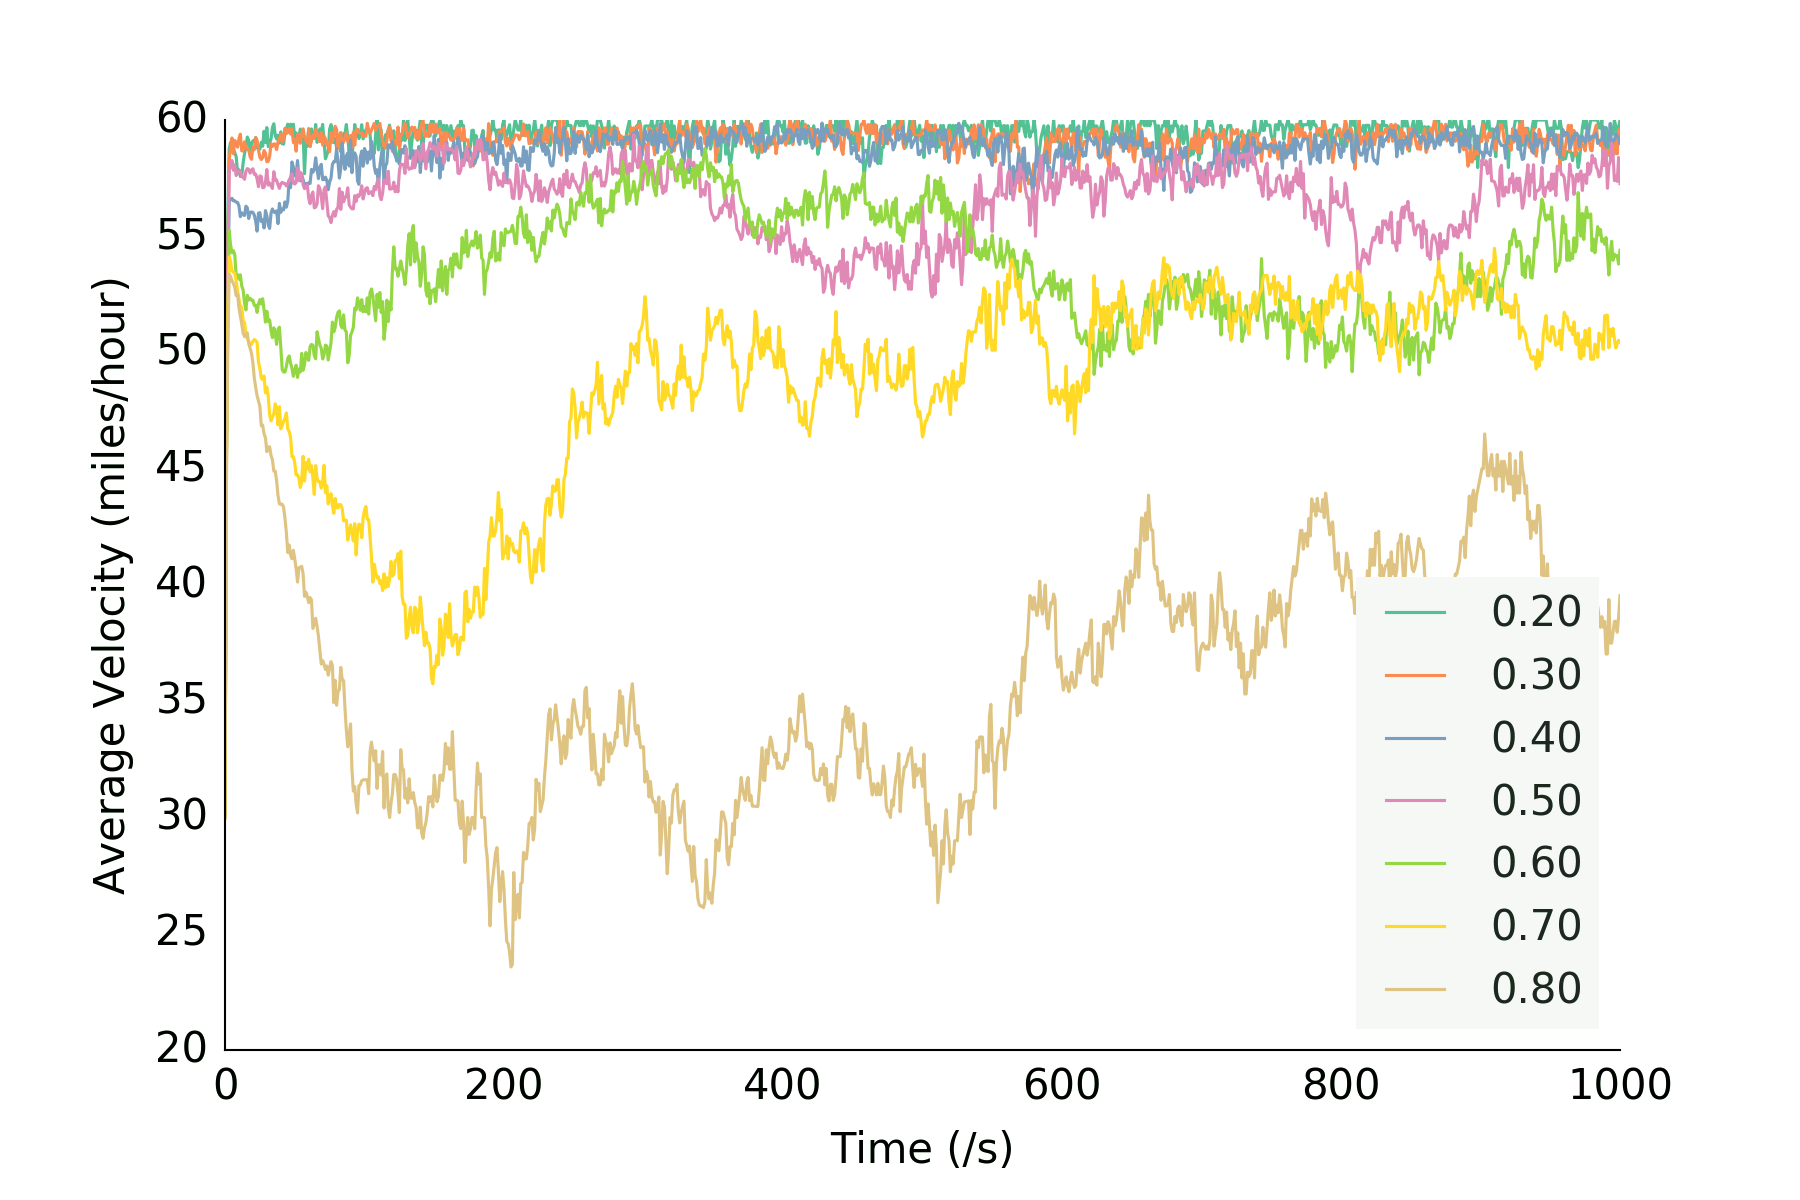
\includegraphics[width=7cm]{tv1.png}
							\caption{Non-self-driving}
						\end{minipage}%
						\begin{minipage}[H]{0.5\linewidth}
							\centering
							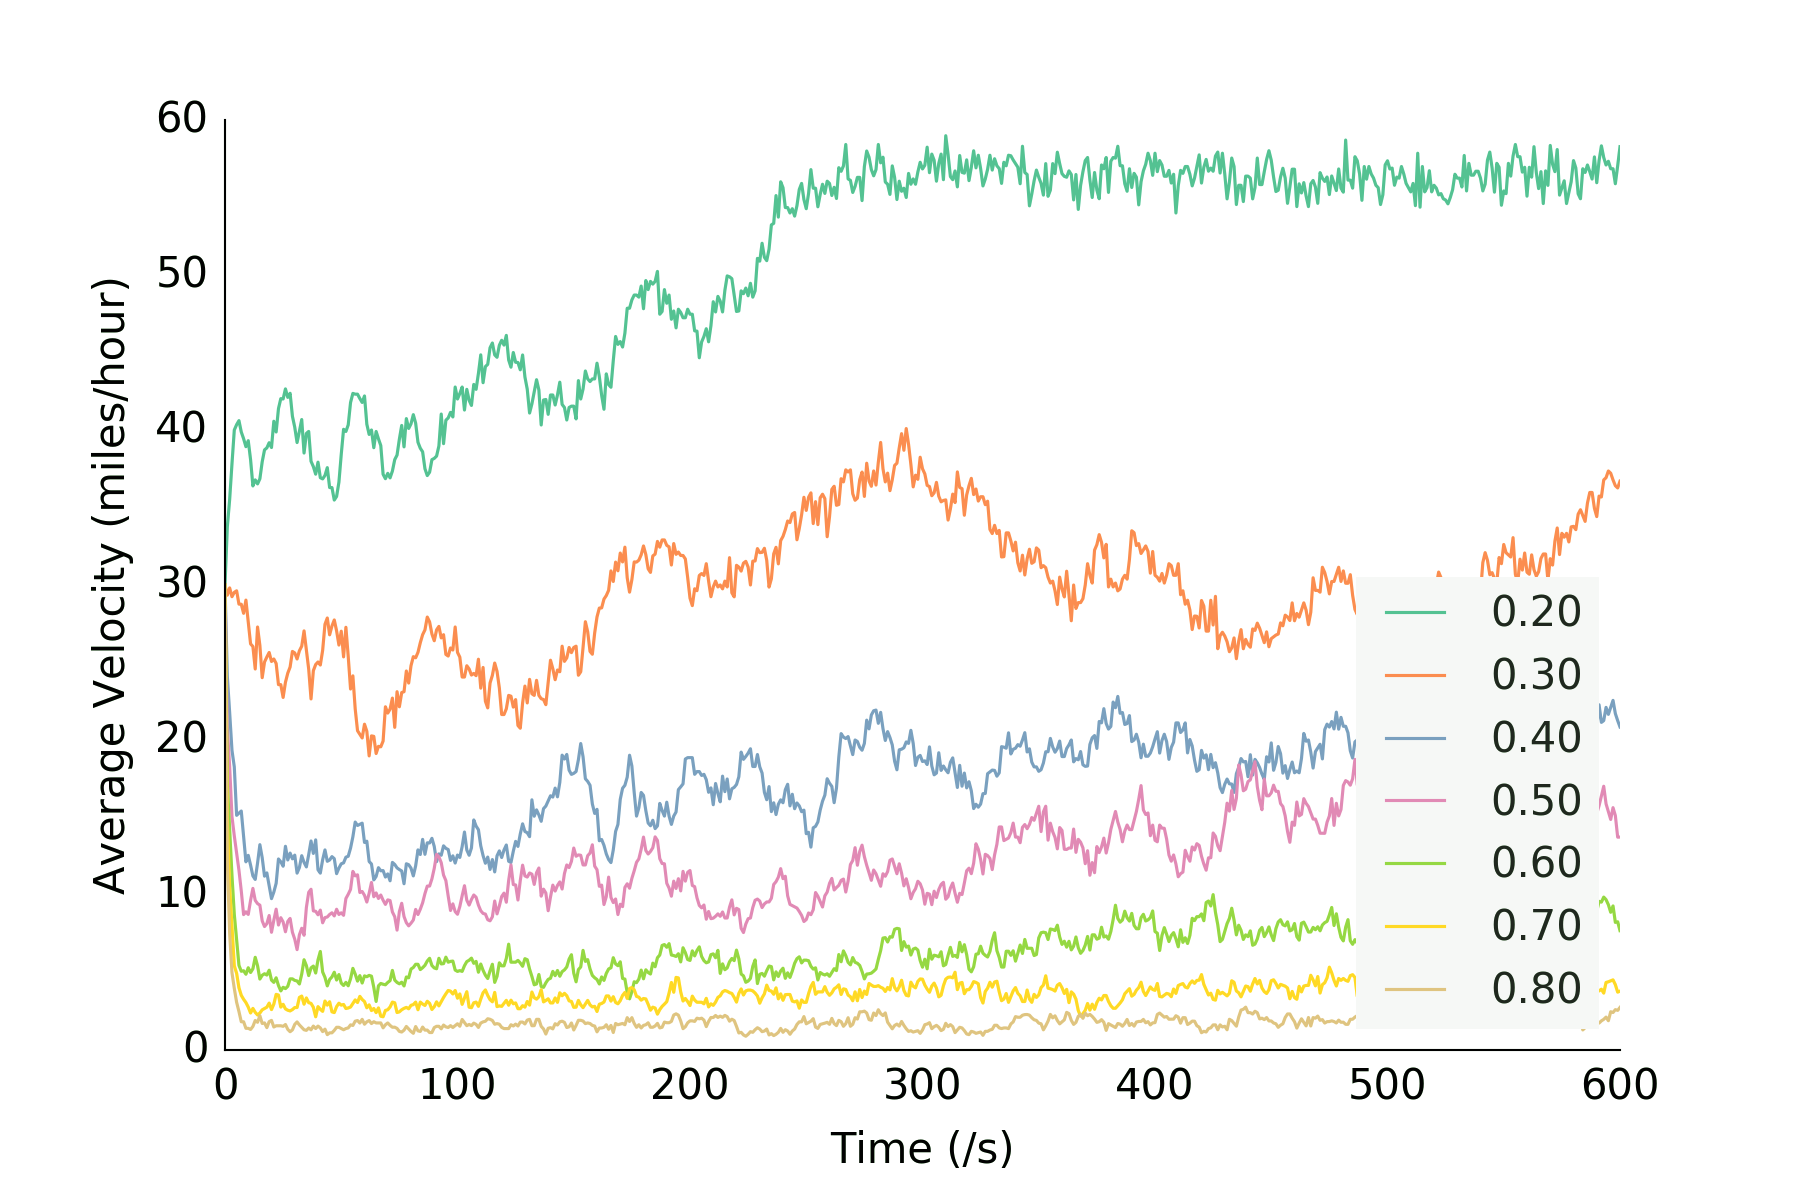
\includegraphics[width=7cm]{tv2.png}
							\caption{Self-driving}
						\end{minipage}
					\end{figure}
					In the graph, self-driving cars use less time to speed up and maintain the high velocity in next period of time. Non-self-driving cars need longer time to speed up and change the speed randomly in next period of time. At the same time, when the percentage of self-driving cars is low, for example 20\%, we find the no obvious difference between self-driving and non-self-driving behavior. Only if the percentage becomes larger, we could find obvious effect on velocity.

				\noindent \textbf{Comparison in density-flow}

					Traffic flow defines as the number of vehicles in a period of time.
					\begin{equation}
						Traffic Flow = \frac{Volume}{Duration}
					\end{equation}
					\begin{figure}[H]
						\begin{minipage}[H]{0.5\linewidth}
							\centering
							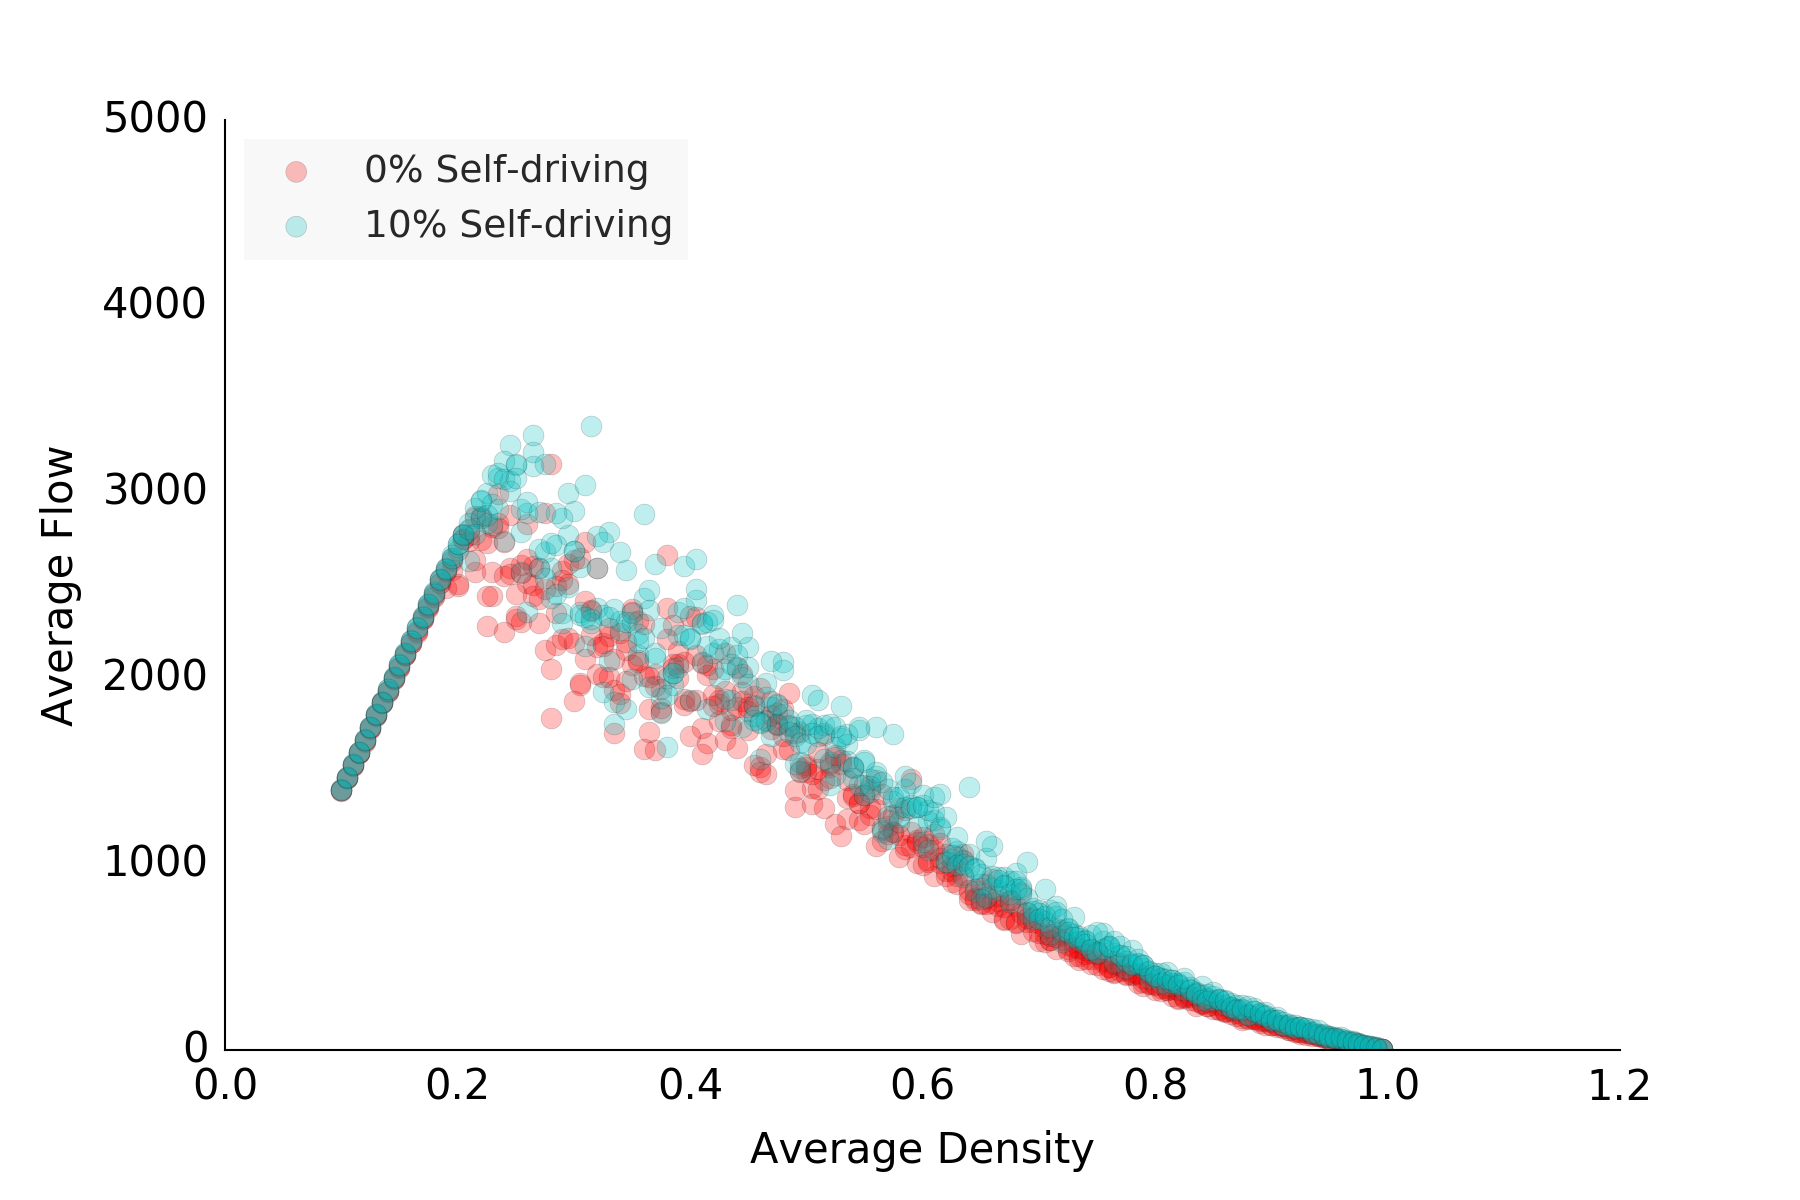
\includegraphics[width=7cm]{df1.png}
						\end{minipage}%
						\begin{minipage}[H]{0.5\linewidth}
							\centering
							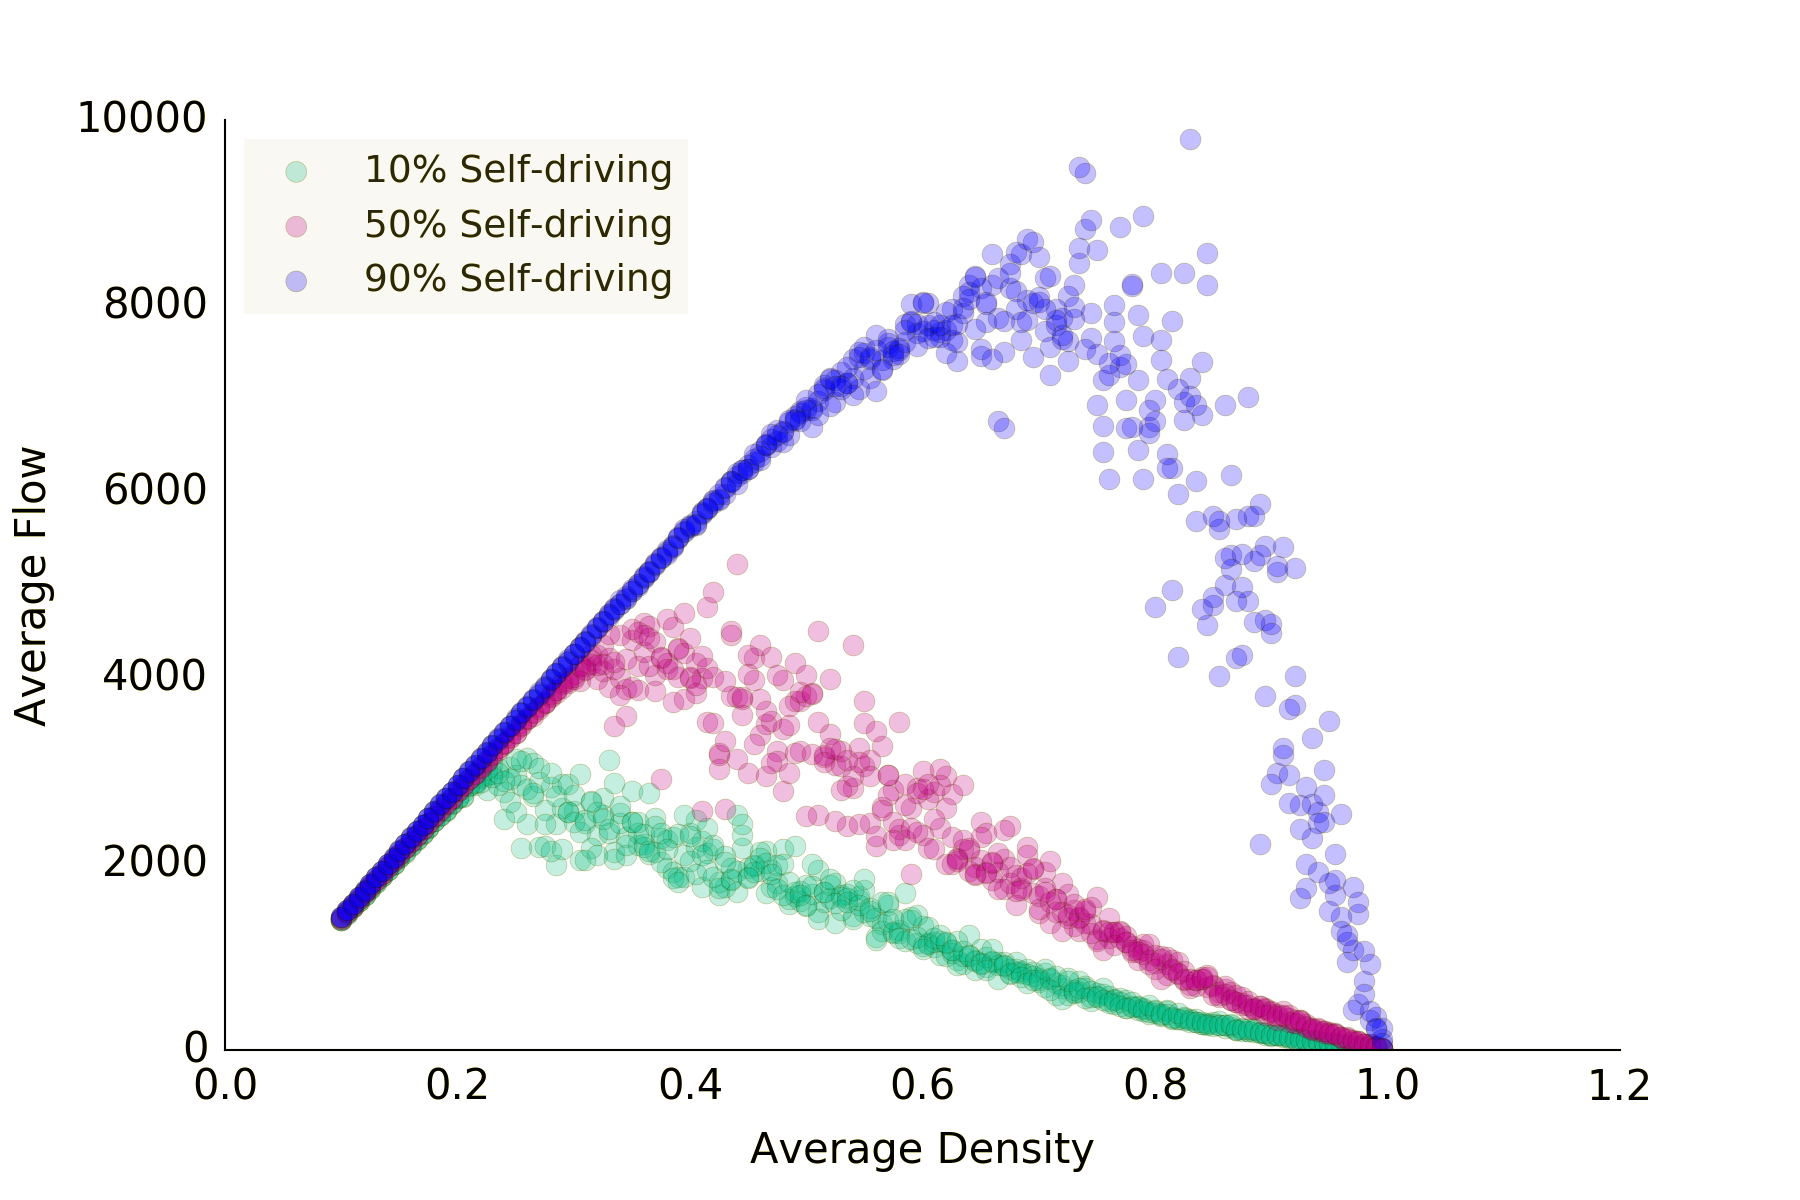
\includegraphics[width=7cm]{df2.png}
						\end{minipage}
						\caption{Density - Flow}
					\end{figure}
					In the figure, we find the same solution with it above that when the percentage of self-driving >50\%, effect will be vivid. When the density is around 0.2, traffic flow will increase to the tipping point. After the tipping point, the traffic flow will gradually decrease. With increase of percentage, other curves which use smaller percent envelope in the curve which uses larger percent.
			\subsubsection{Prediction}
				We predict the self-driving behavior in real road situation by considering:
				\begin{itemize}
					\item Data of probability of entry, which contains three factors to influence the results.
					\item Influence factors of self-driving situation.
				\end{itemize}
				And stimulate the self-driving in Route 5, we get the figure below:
				\begin{figure}[H]
					\begin{center}
						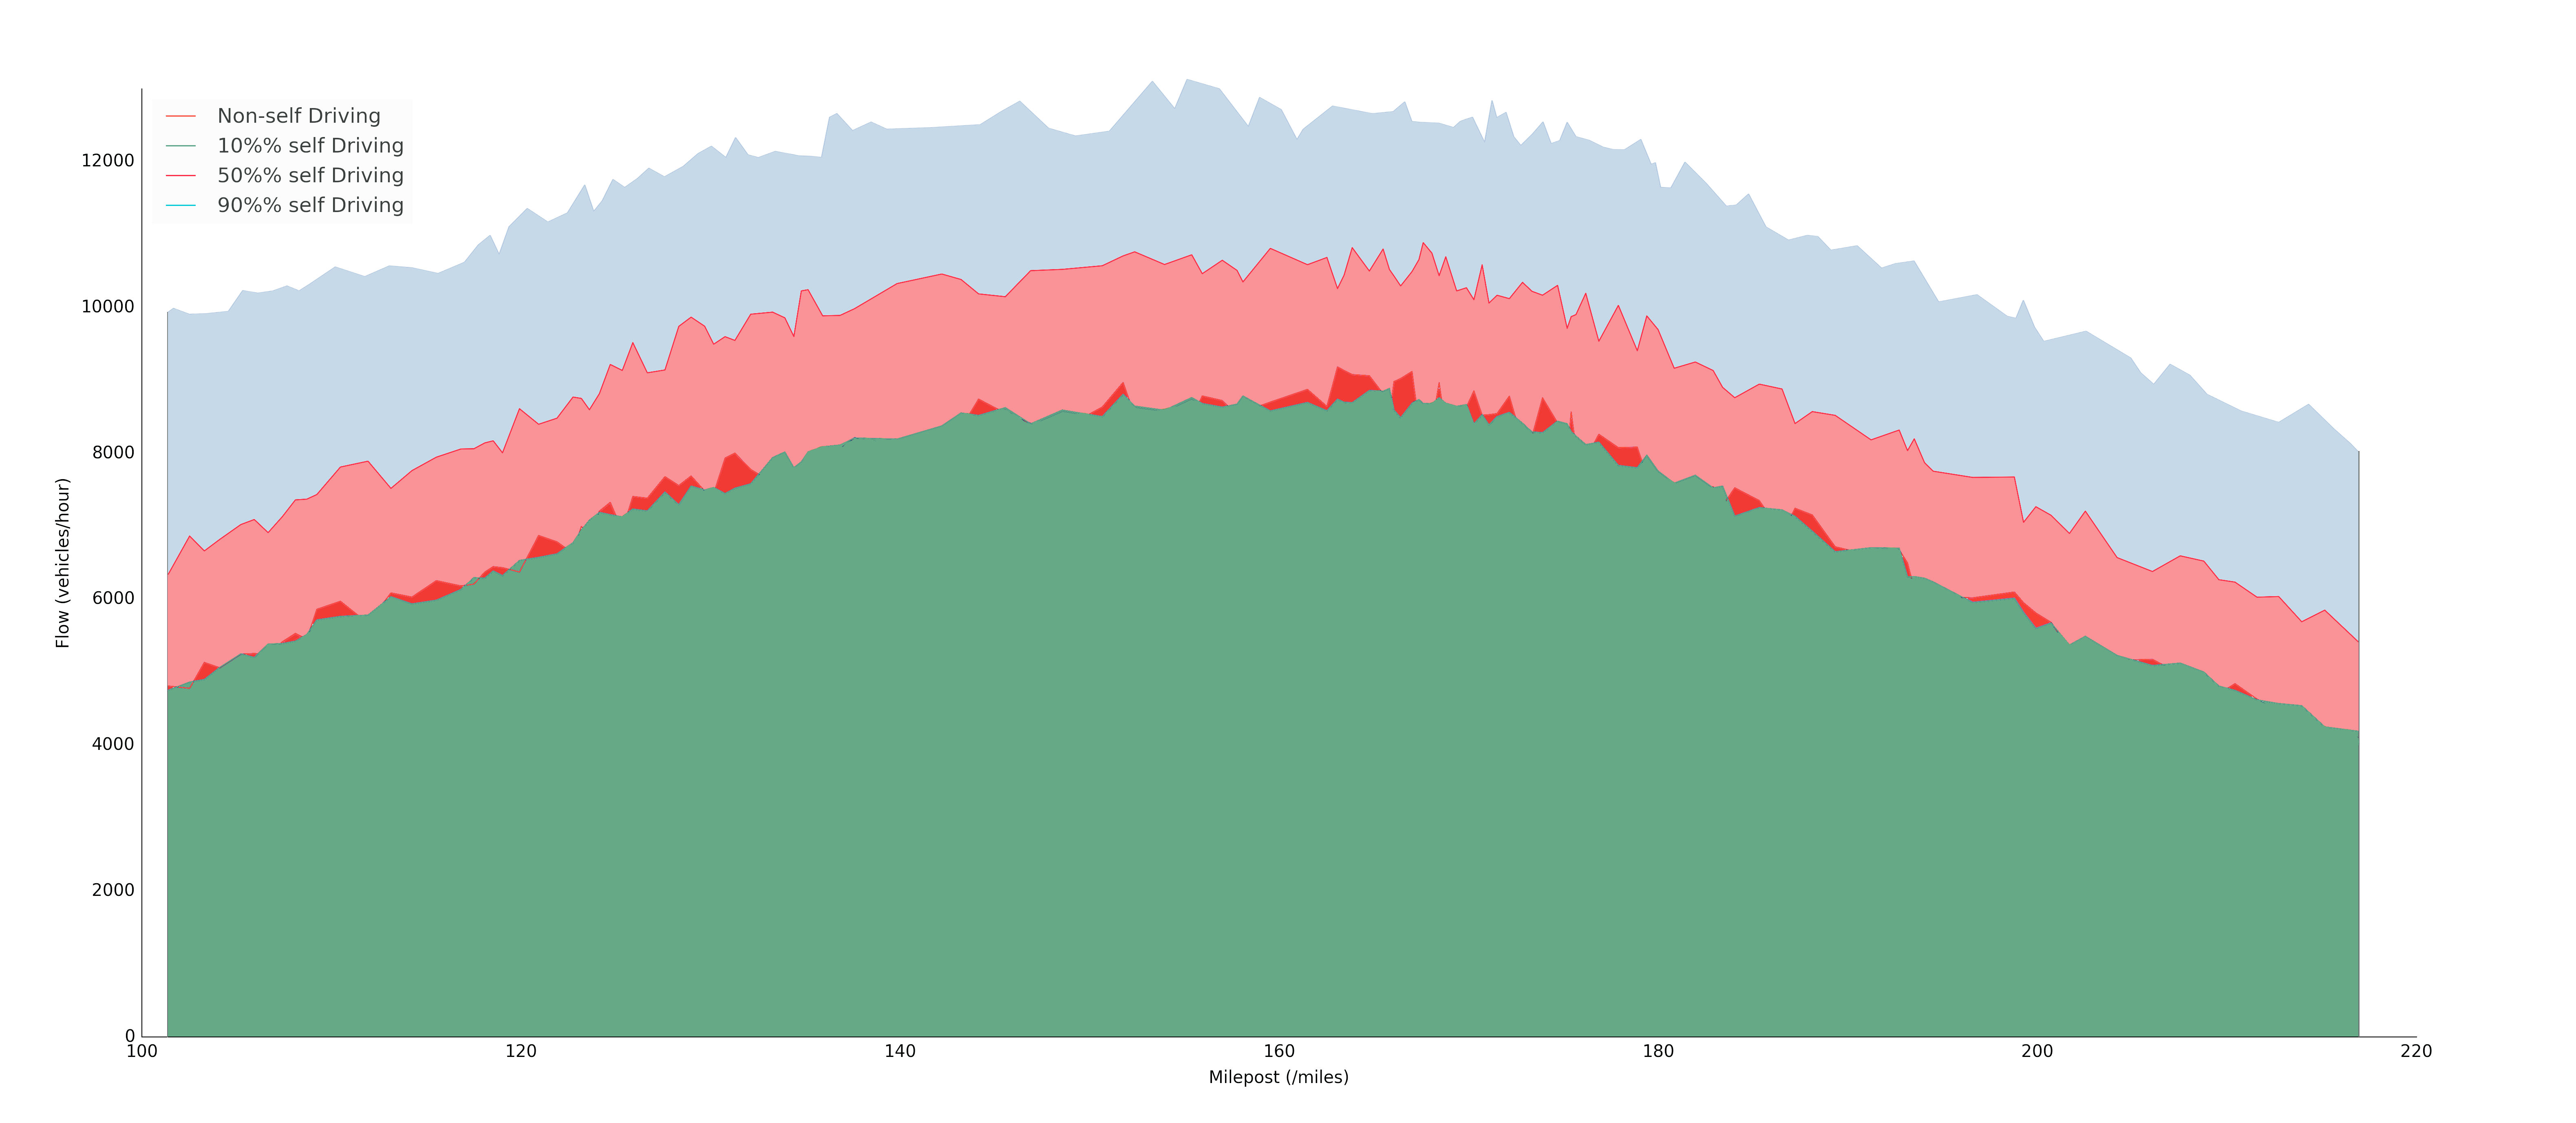
\includegraphics[width=10cm]{aaa.png}
						\caption{Prediction of self-driving}
					\end{center}
				\end{figure}


		\subsection{Evaluating Equilibria}
			We create an evaluating model to analyze the effect of self-driving cars. The factors are the same as we talked above. The model is:
			\begin{equation}
				Score = \frac{A}{1 + e^{\mu(\varepsilon_{1} D_{peaking} + \varepsilon_{2} D_{interstate} + \varepsilon_{3} D_{junction}) p_{i}^{\varepsilon_{4}}}}
			\end{equation}

			So in the model, when the percentage of self-driving increases with a small growth rate, the score will grow slowly. After a point of percentage, the score grow rapidly to reach the full score. But while the percentage is getting close to the full score, it will develop slowly again, which always reaching to the full but cannot get.
			\begin{figure}[H]
				\begin{center}
					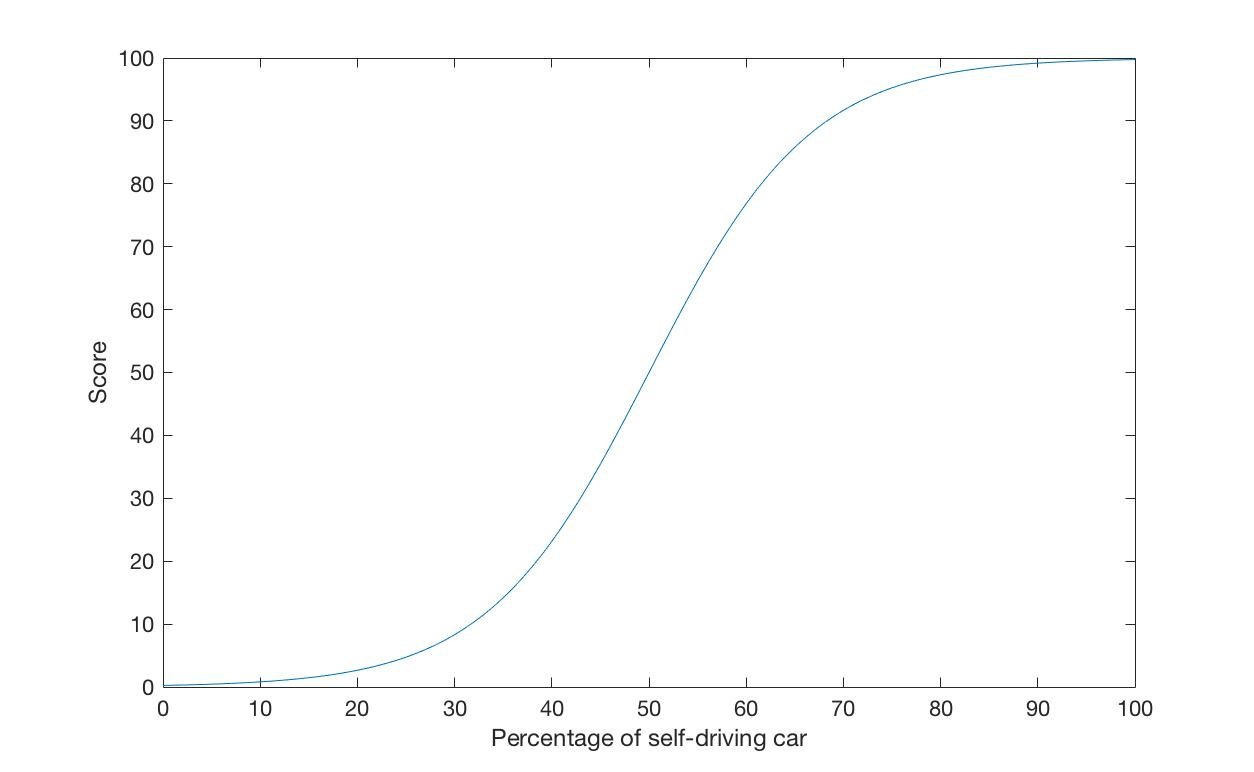
\includegraphics[width=10cm]{score1.jpg}
					\caption{The curve of $Score$}
				\end{center}
			\end{figure}

			The result is equilibria does not exist in theory. However, we didn't consider the implement of policy and the cost of the replacement. After adding these two influencing factors, the evaluating model is much closer to the actual situation. Here is the expanded model below:

			\begin{equation}
				Score = \frac{A}{1 + e^{\mu(\varepsilon_{1} D_{peaking} + \varepsilon_{2} D_{interstate} + \varepsilon_{3} D_{junction}) p_{i}^{\varepsilon_{4}}}} - \varphi(p_{i}) + D_{p} (\xi(p_{i}) - \delta(p_{i}))
			\end{equation}
			\begin{table}[H]
				\caption{Extra Notations in Expanded Evaluating Model}
				\begin{center}
					\begin{longtable}{m{80pt}<{\centering} | m{280pt}}
						\hline%----------------------------------------------------------------------------------------------------------
						Notations 			& 	Definition \\
						\hline%----------------------------------------------------------------------------------------------------------
						$\varphi(p_{i})$ 	&	The effect cause by the cost of replacing the traditional cars with self-driving cars.\\
						\hline%----------------------------------------------------------------------------------------------------------
						$D_{p}$				&	Whether there is policies encouraging popularizing self-driving car. If exist, the value of $D_{p}$ is 1.\\
						\hline%----------------------------------------------------------------------------------------------------------
						$\xi(p_{i})$		&	The effect of policy implementation.\\
						\hline%----------------------------------------------------------------------------------------------------------
						$\delta(p_{i})$		&	The effect cause by the time required for the implementation of the policy.\\
						\hline%----------------------------------------------------------------------------------------------------------
					\end{longtable}
				\end{center}
			\end{table}
			In this new model, the time of policy implement plays an important role. If the implement costs several years to change the percentage of self-driving car, the effect of the self-driving car is not so obvious in the graph. And then, self-driving cars, as automatic and intelligent machines, may cost more money than non-self-driving cars, which will influence the effect as well. But with the time goes, the cost of both self-driving and non-self-driving cars will decrease gradually.So the score cruve has the tipping point.

			\begin{figure}[H]
				\begin{center}
					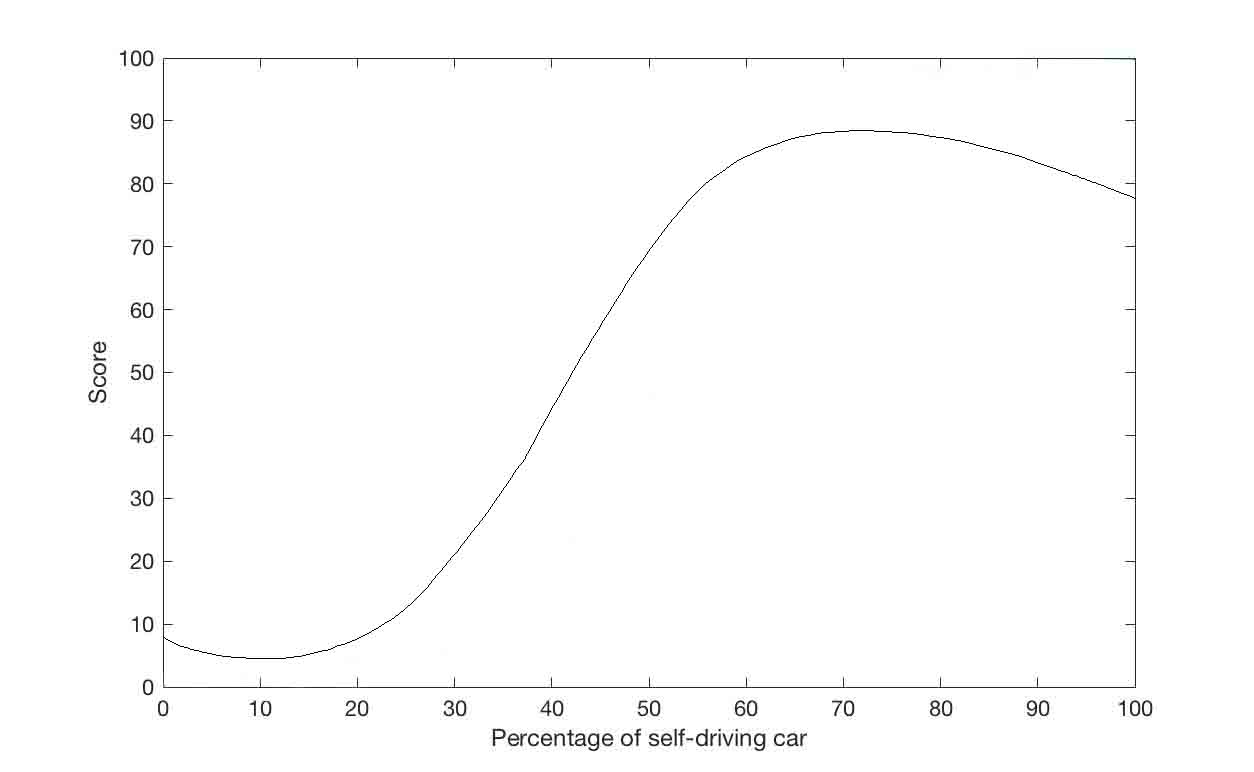
\includegraphics[width=10cm]{score2.jpg}
					\caption{The curve of $Score$ after expanded}
				\end{center}
			\end{figure}

		\subsection{Self-driving behavior in divided lanes}
			Based on the performance of self-driving behavior, the higher percentage of self-driving usage is the larger traffic flow and more vividly efficiency will be.

			We divide the highway into accommodation lane for self-driving car and common lane for non-self-driving car. Define that the car in both lane cannot travel to each other. So the interaction with self-driving cars and non-self-driving car disappears. 
			\begin{figure}[H]
				\begin{center}
					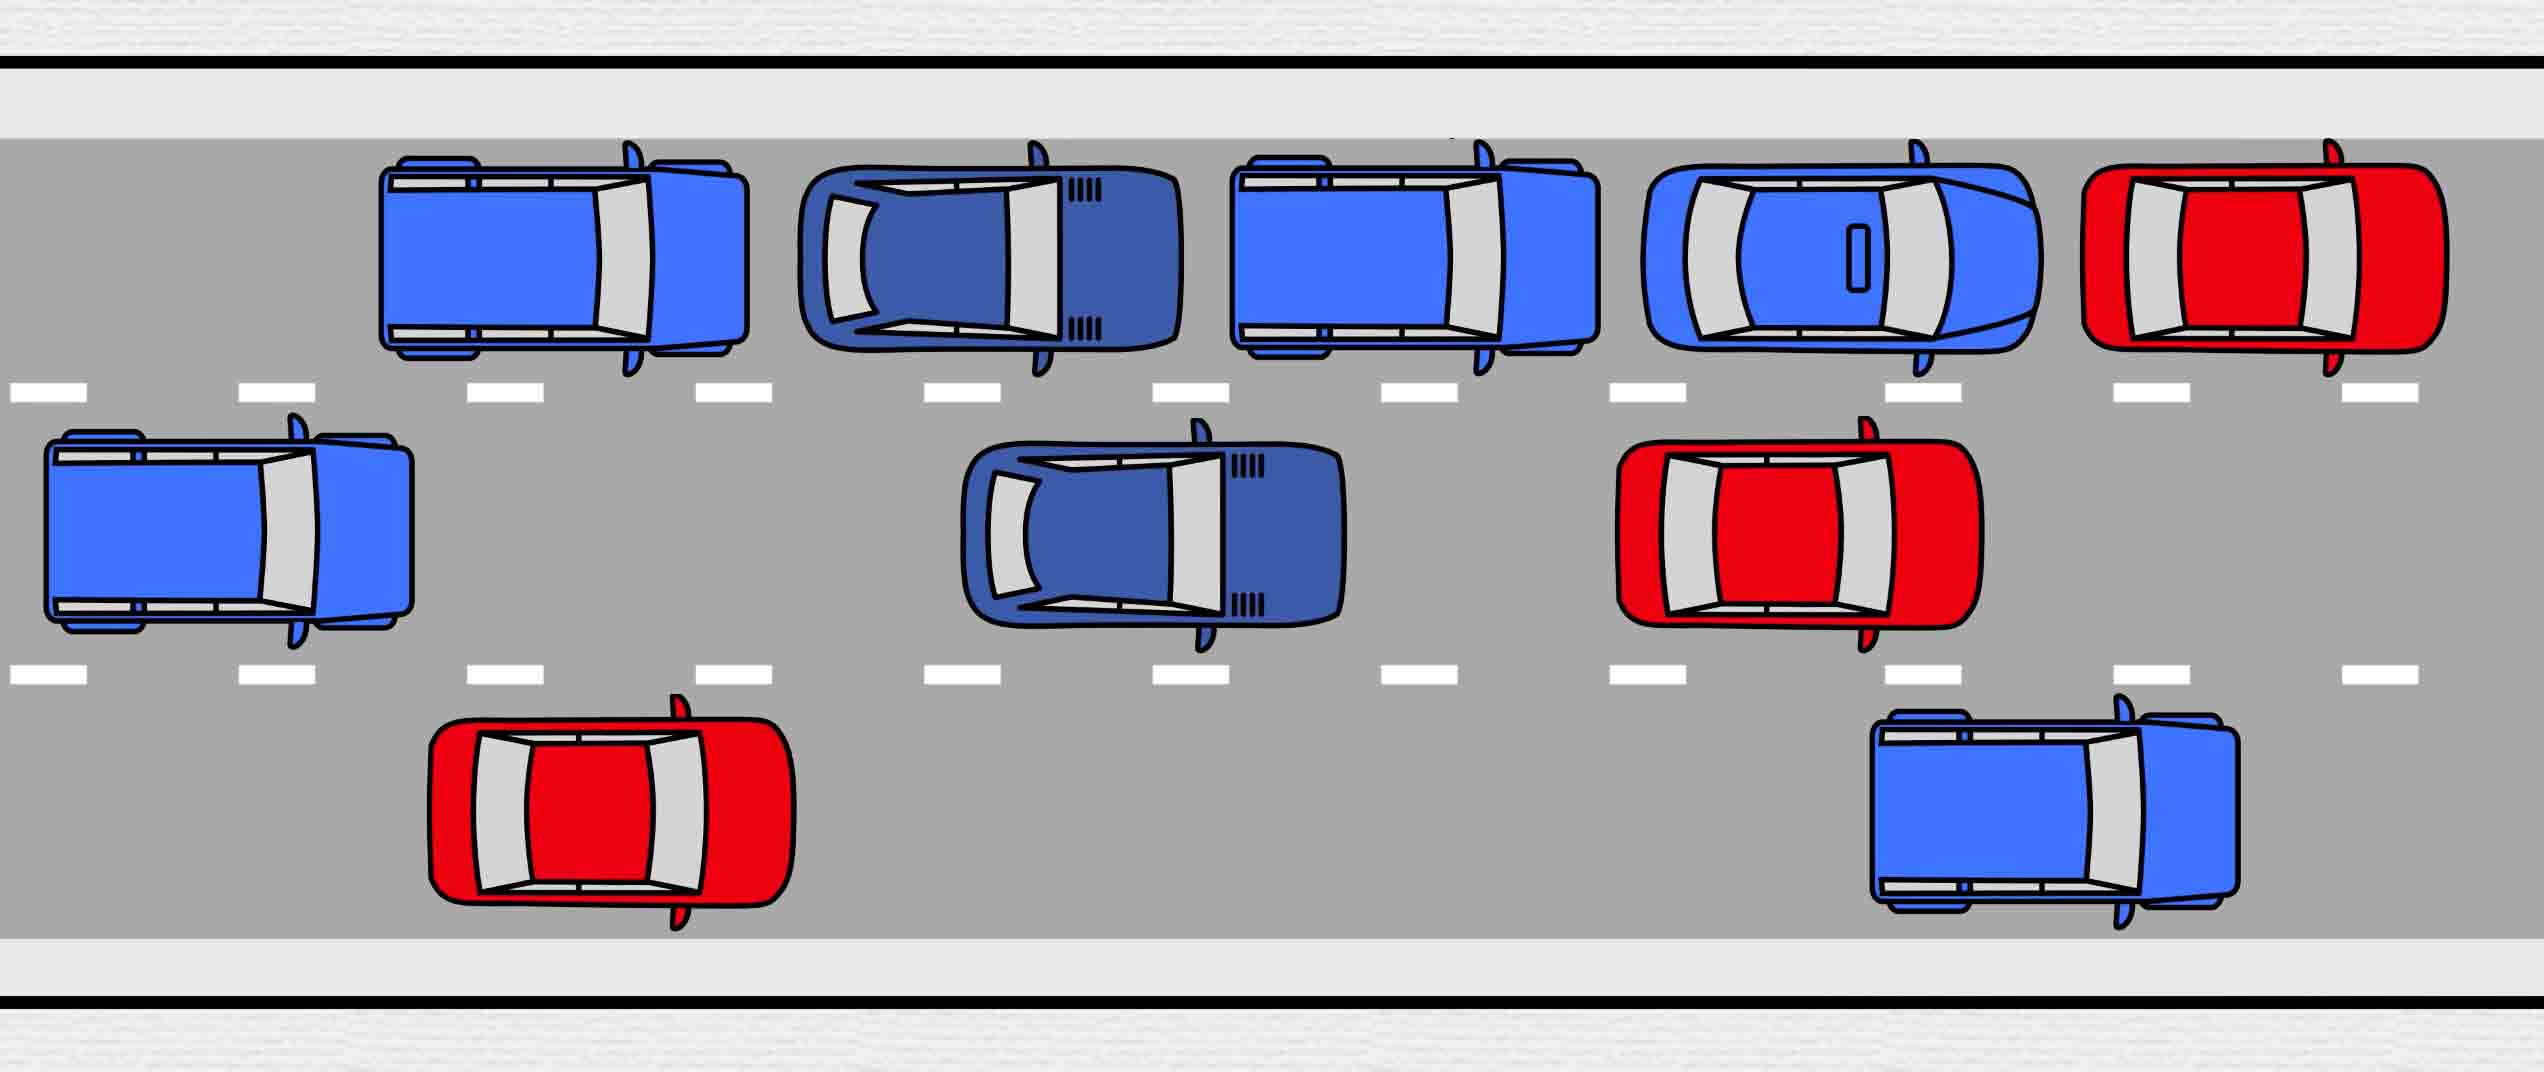
\includegraphics[width=14cm]{divided.jpg}
					\caption{Behavior on divided lanes}
				\end{center}
			\end{figure}

			Then we can analyze the situation of traffic performance respectively.

			\noindent \textbf{Non-self-driving situation}

			Suit the rules in standard N-S model and modified VDR model above. But paying attention to the number of lanes after dividing the highway, the ratio of entry will be smaller than before limiting to the number of lanes.

			\noindent \textbf{Self-driving situation}

			In this case the percentage of self-driving usage is 100\%. So, we just consider the cooperation between self-driving cars. Gap between front car and following car approximately is 0. We can see it as a train carriage end to end .If more lanes are specialized for self-driving cars, the traffic flow will be larger and larger.

			Comparing two situations with the density-flow, we can find that there is great different between self-driving car and non-self-driving car. If governor issues the policy to divided highway for self-driving cars, the capacity of traffic will be exactly improved.   


	\section{Sensitivity Analysis}
		A stable model should withstand the change of variables. We calculate the changing of parameter and get the sheet below.
		\newpage
		\begin{center}
			Table 8: The variation of parameters
		\end{center}
		\begin{figure}[H]
			\begin{center}
				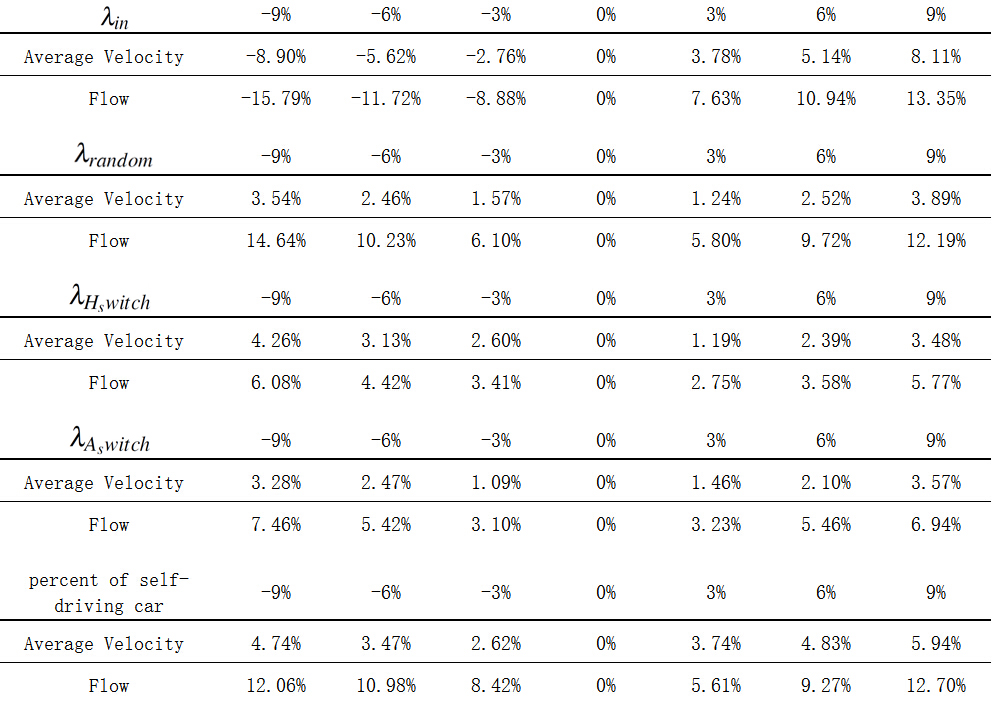
\includegraphics[width=13cm]{sen.jpg}
				\caption*{}
			\end{center}
		\end{figure}

		In the sheet, we change the parameter: probability of entry, probability of randomization, the probability of changing lanes and different $v_{max}$. At the same time, we consider the case of self-driving behavior so that we should take percentage of self-driving car into discussion. The percentage of self-driving car is changing around the tipping point throughout the evaluating system. It is obvious that our solution waves in a reasonable range.


	\section{Conclusion}
		\subsection{Result}
			According to the model establishment and simulation, we can draw conclusion as follows: 
			\begin{itemize}
				\item Self-driving cars can performance much better than non-self-driving cars. By using self-driving car, there will be less possibility of traffic jam occur on highways. 
				\item When mix self-driving cars with non-self-driving cars, with the percentage of self-driving car increase, the traffic capacity of highways will larger and larger. However, this conclusion is under the precondition that we consider driving behavior and road condition only.
				\item When take costs and policies into consideration, only the percentage is within a specific range can its growth lead to a obvious effect.
			\end{itemize}

		\subsection{Evaluating the Model}
			Like any model, our model has its own strengths and weaknesses. Some of major points are presented below. 

			\subsubsection{Strengths}
				\begin{itemize}
					\item Use the N-S model to simulate the traffic performance and simplify the highway into a set of cells. In addition, we analyze relation between time-space, time- velocity and density-flow in different kind of driving behavior.
					\item Connect the real traffic situation with our model and try to fix the real situation. Give the certain parameter to stimulate the real traffic environment.
					\item In modified model, we consider more reliable factors which affect the traffic flow and add them into our model. And it suits the real situation well. Expand to the situation of self-driving and predict the solution.
					\item We import an evaluating system to describe the utility of change in percentage of self-driving usage. Suppose the influence of policy and cost at the same time.
					\item We use Matlab to test different situation. Our model withstands variables change.
					\item Use several figures to describe our model so the conclusion looks obvious.
				\end{itemize}
			\subsubsection{Weaknesses}
				\begin{itemize}
					\item Limit to the data of real situation, we cannot get accurate number of volume in one hour and how long the peaking hour is.
					\item Density is unknown in the question so we assume several densities to line in the figure and get the relation of the traffic flow. And they are beginning densities. But in reality, densities are different in lanes.
					\item We use the solution of non-self-driving car to stimulate the condition of self-driving car. However there is no deny that disparity exists and unknown.
					\item Do not consider the probability of accidents happen, which may have great effect on traffic flow.
					\item Simplify the lane in both-way traffic by weighting the number of lanes. But in real traffic, density and flow are different in increasing direction and decreasing direction.
					\item We select one road to stimulate and speculate. It is possible that the solution may not suit other four highways.
				\end{itemize}

	\section{Further Study}
		Different people have different tendencies to randomization. In general, a more experienced driver seldom slow down his speed in highways. We can guess the percentage of experienced drivers in highway to change the probability of randomization. Classify the experienced driver and unexperienced driver help us to calculate the interaction between self-driving car and different kind of drivers.

		Consider the probability of accident. It is possible that accident happen in peaking hour and intersection with other roads. Accidents will have great effect on traffic flow and speed. If there is an accident happening, the following car must slow down and change lane, which will lead to traffic jam sooner or later.

		Consider people’s emotion whether the driver have aggressive or competing behavior in highway. It depends on the condition of road, interaction with surrounding cars and the time of driving.

		After a long time of driving, people may have aggressive behavior in highways.

		When traffic flow is large, it is possible that several cars travel parallel and drivers may compete with each other. 
		If there is a traffic jam, people’s emotion change with the time to regain.

		Age and gender may affect people’s attitude to self-driving car. 

		The elderly may have limited in driving ability and willing to buy the self-driving car. Women want to purchasing self-driving car for lack of driving experience. 

		However, some people do not want to use self-driving car because it will less interesting in driving time so that at the beginning of policy, not so many people want to buy the self-driving cars. 

		Usage of self-driving car also limits to personal income. Rich people will possibly have aspiration on purchasing the self-driving car. Self-driving car may generate gradually and the cost may decline to satisfy people afford.

	\newpage
	\titleformat*{\section}{\centering\huge}
	\section*{Letter to the Governor}
	\addcontentsline{toc}{section}{Letter to the Governor}
		\noindent Dear Sir or Madam: 

		Upon hearing that the Governor of the state of Washington has asked for analysis of the effects of allowing cooperating, self-driving cars on the roads in Thurston, Pierce, King, and Snohomish counties, we are glad for the news because we have indeed suffered from the traffic jam in highway for a long time, for the reason that traffic capacity is limited in many regions of the United States due to the number of lanes of roads. The volume of traffic exceeds the designed capacity of the road networks, particularly pronounced on Interstate Routes and State Routes.

		These days, our team researched and compared the effect of using self-driving cars to using non-self-driving cars. Meanwhile, we also analyzed the effect of mixed lanes, where self-driving cars and non-self-driving cars travel together, and divided lanes which self-driving cars have a specialized lane to travel. We hope it can give assistance for you to make the policy and regulation.

		Inspired by the Cellular Automata Simulation, we established the model of non-self-driving cars in highway. According to adding the unique variables and parameter, we easily got the model of self-driving cars. We found that the more percentage of usage of self-driving car, the greater counts of volume it will be. Self-driving car can perfectly cooperate with each other to avoid the traffic jam and accidents. So, the governor can advocate the using of self-driving car by publish the policy to cut down the expense of buying self-driving cars by providing subsidy or encourage the auto industry to produce more economic self-driving cars.

		Then, we expanded the model to compare the mixed lane and divided lane. We got the conclusion that if the government constructs specialized lane in the high way, the volume of lane will be larger. In an extreme assumption, if all the lanes are for self-driving cars (In another word, self-driving cars replace non-self-driving cars.) So government can make full use of this point to divide the highway to smooth the efficient traffic.

		We established an evaluation mechanism to evaluate equilibria of the self-driving model at the same time. Equilibria depends on several factors, one of the most important factor is the time need of the policy in force. In the mechanism, the shorter time use, the earlier the traffic condition will improve. So, we strongly suggest government to take immediate action to advocate the usage of self-driving cars.
		We hope it sincerely that our solution can help you to list the policy to improve the traffic condition in highways.
		\begin{flushright}
		Yours sincerely
		\end{flushright}

	\newpage
	\begin{thebibliography}{99}
		\bibitem{1}\url{http://www.google.com/selfdrivingcar/}
		\bibitem{2}Ning W U, Brilon W. Cellular Automata for Highway Traffic Flow Simulation[C]// transportation and traffic theory: papers presented at the abbreviated presentation sessions. 1999.
		\bibitem{3}Schadschneider A. Cellular automata models of highway traffic[J]. Physica A Statistical Mechanics \& Its Applications, 2006, 372(1):142-150.
		\bibitem{4}Ding D. Modeling and simulation of highway traffic using a cellular automaton approach[J]. 2012.
		\bibitem{5}Michael Sivak, Brandon Schoettle. Road Safety with Self-Driving Vehicles: General Limitations and Road Sharing with Conventional Vehicles[J]. 2015.
	\end{thebibliography}
\end{document}


